%%%%%%%%%%%%%%%%%%%%%%%%%%%%%%%%%%%%%%%%%
%  My documentation report
%  Objetive: Explain what I did and how, so someone can continue with the investigation
%
% Important note:
% Chapter heading images should have a 2:1 width:height ratio,
% e.g. 920px width and 460px height.
%
%%%%%%%%%%%%%%%%%%%%%%%%%%%%%%%%%%%%%%%%%

%----------------------------------------------------------------------------------------
%	PACKAGES AND OTHER DOCUMENT CONFIGURATIONS
%----------------------------------------------------------------------------------------

\documentclass[12pt,ngerman, fleqn]{book} % Default font size and left-justified equations

\usepackage[top=3cm,bottom=3cm,left=3.2cm,right=3.2cm,headsep=10pt,letterpaper]{geometry} % Page margins

\usepackage{xcolor} % Required for specifying colors by name
\definecolor{ocre}{RGB}{52,177,201} % Define the orange color used for highlighting throughout the book

%Imojis :)
%\usepackage{coloremoji}

%Euro sign
\usepackage{german}
\usepackage{eurosym}

%figure wrap
\usepackage{wrapfig}

%Special charachters
\usepackage{pifont}

% for figure grouping
\usepackage{subcaption}
\usepackage{graphicx}

% Font Settings
\usepackage{avant} % Use the Avantgarde font for headings
%\usepackage{times} % Use the Times font for headings
\usepackage{mathptmx} % Use the Adobe Times Roman as the default text font together with math symbols from the Symbol, Chancery and Computer Modern fonts

%\usepackage{microtype} % Slightly tweak font spacing for aesthetics
\usepackage[utf8]{inputenc} % Required for including letters with accents 
\usepackage[T1]{fontenc} % Use 8-bit encoding that has 256 glyphs

% Bibliography
%\usepackage[style=alphabetic,sorting=nyt,sortcites=true,autopunct=true,babel=hyphen,hyperref=true,abbreviate=false,backref=true,backend=biber]{biblatex}
%\addbibresource{bibliography.bib} % BibTeX bibliography file
%\defbibheading{bibempty}{}

\usepackage{csquotes}
\usepackage[style=verbose-ibid,backend=bibtex]{biblatex}
\addbibresource{bibliography.bib}

%----------------------------------------------------------------------------------------
%	VARIOUS REQUIRED PACKAGES
%----------------------------------------------------------------------------------------

\usepackage{titlesec} % Allows customization of titles

\usepackage{graphicx} % Required for including pictures
\graphicspath{{Pictures/}} % Specifies the directory where pictures are stored

\usepackage{lipsum} % Inserts dummy text

\usepackage{tikz} % Required for drawing custom shapes

\usepackage[german, english]{babel} % English language/hyphenation

\usepackage{enumitem} % Customize lists
\setlist{nolistsep} % Reduce spacing between bullet points and numbered lists

\usepackage{booktabs} % Required for nicer horizontal rules in tables

\usepackage{eso-pic} % Required for specifying an image background in the title page

%----------------------------------------------------------------------------------------
%	MAIN TABLE OF CONTENTS
%----------------------------------------------------------------------------------------

\usepackage{titletoc} % Required for manipulating the table of contents

\contentsmargin{0cm} % Removes the default margin
% Chapter text styling
\titlecontents{chapter}[1.25cm] % Indentation
{\addvspace{15pt}\large\sffamily\bfseries} % Spacing and font options for chapters
{\color{ocre!60}\contentslabel[\Large\thecontentslabel]{1.25cm}\color{ocre}} % Chapter number
{}  
{\color{ocre!60}\normalsize\sffamily\bfseries\;\titlerule*[.5pc]{.}\;\thecontentspage} % Page number
% Section text styling
\titlecontents{section}[1.25cm] % Indentation
{\addvspace{5pt}\sffamily\bfseries} % Spacing and font options for sections
{\contentslabel[\thecontentslabel]{1.25cm}} % Section number
{}
{\sffamily\hfill\color{black}\thecontentspage} % Page number
[]
% Subsection text styling
\titlecontents{subsection}[1.25cm] % Indentation
{\addvspace{1pt}\sffamily\small} % Spacing and font options for subsections
{\contentslabel[\thecontentslabel]{1.25cm}} % Subsection number
{}
{\sffamily\;\titlerule*[.5pc]{.}\;\thecontentspage} % Page number
[] 

%----------------------------------------------------------------------------------------
%	MINI TABLE OF CONTENTS IN CHAPTER HEADS
%----------------------------------------------------------------------------------------

% Section text styling
\titlecontents{lsection}[0em] % Indendating
{\footnotesize\sffamily} % Font settings
{}
{}
{}

% Subsection text styling
\titlecontents{lsubsection}[.5em] % Indentation
{\normalfont\footnotesize\sffamily} % Font settings
{}
{}
{}
 
%----------------------------------------------------------------------------------------
%	PAGE HEADERS
%----------------------------------------------------------------------------------------

\usepackage{fancyhdr} % Required for header and footer configuration

\pagestyle{fancy}
\renewcommand{\chaptermark}[1]{\markboth{\sffamily\normalsize\bfseries\chaptername\ \thechapter.\ #1}{}} % Chapter text font settings
\renewcommand{\sectionmark}[1]{\markright{\sffamily\normalsize\thesection\hspace{5pt}#1}{}} % Section text font settings
\fancyhf{} \fancyhead[LE,RO]{\sffamily\normalsize\thepage} % Font setting for the page number in the header
\fancyhead[LO]{\rightmark} % Print the nearest section name on the left side of odd pages
\fancyhead[RE]{\leftmark} % Print the current chapter name on the right side of even pages
\renewcommand{\headrulewidth}{0.5pt} % Width of the rule under the header
\addtolength{\headheight}{2.5pt} % Increase the spacing around the header slightly
\renewcommand{\footrulewidth}{0pt} % Removes the rule in the footer
\fancypagestyle{plain}{\fancyhead{}\renewcommand{\headrulewidth}{0pt}} % Style for when a plain pagestyle is specified

% Removes the header from odd empty pages at the end of chapters
\makeatletter
\renewcommand{\cleardoublepage}{
\clearpage\ifodd\c@page\else
\hbox{}
\vspace*{\fill}
\thispagestyle{empty}
\newpage
\fi}

%----------------------------------------------------------------------------------------
%	THEOREM STYLES
%----------------------------------------------------------------------------------------

\usepackage{amsmath,amsfonts,amssymb,amsthm} % For math equations, theorems, symbols, etc

\newcommand{\intoo}[2]{\mathopen{]}#1\,;#2\mathclose{[}}
\newcommand{\ud}{\mathop{\mathrm{{}d}}\mathopen{}}
\newcommand{\intff}[2]{\mathopen{[}#1\,;#2\mathclose{]}}
\newtheorem{notation}{Notation}[chapter]

%%%%%%%%%%%%%%%%%%%%%%%%%%%%%%%%%%%%%%%%%%%%%%%%%%%%%%%%%%%%%%%%%%%%%%%%%%%
%%%%%%%%%%%%%%%%%%%% dedicated to boxed/framed environements %%%%%%%%%%%%%%
%%%%%%%%%%%%%%%%%%%%%%%%%%%%%%%%%%%%%%%%%%%%%%%%%%%%%%%%%%%%%%%%%%%%%%%%%%%
\newtheoremstyle{ocrenumbox}% % Theorem style name
{0pt}% Space above
{0pt}% Space below
{\normalfont}% % Body font
{}% Indent amount
{\small\bf\sffamily\color{ocre}}% % Theorem head font
{\;}% Punctuation after theorem head
{0.25em}% Space after theorem head
{\small\sffamily\color{ocre}\thmname{#1}\nobreakspace\thmnumber{\@ifnotempty{#1}{}\@upn{#2}}% Theorem text (e.g. Theorem 2.1)
\thmnote{\nobreakspace\the\thm@notefont\sffamily\bfseries\color{black}---\nobreakspace#3.}} % Optional theorem note
\renewcommand{\qedsymbol}{$\blacksquare$}% Optional qed square

\newtheoremstyle{blacknumex}% Theorem style name
{5pt}% Space above
{5pt}% Space below
{\normalfont}% Body font
{} % Indent amount
{\small\bf\sffamily}% Theorem head font
{\;}% Punctuation after theorem head
{0.25em}% Space after theorem head
{\small\sffamily{\tiny\ensuremath{\blacksquare}}\nobreakspace\thmname{#1}\nobreakspace\thmnumber{\@ifnotempty{#1}{}\@upn{#2}}% Theorem text (e.g. Theorem 2.1)
\thmnote{\nobreakspace\the\thm@notefont\sffamily\bfseries---\nobreakspace#3.}}% Optional theorem note

\newtheoremstyle{blacknumbox} % Theorem style name
{0pt}% Space above
{0pt}% Space below
{\normalfont}% Body font
{}% Indent amount
{\small\bf\sffamily}% Theorem head font
{\;}% Punctuation after theorem head
{0.25em}% Space after theorem head
{\small\sffamily\thmname{#1}\nobreakspace\thmnumber{\@ifnotempty{#1}{}\@upn{#2}}% Theorem text (e.g. Theorem 2.1)
\thmnote{\nobreakspace\the\thm@notefont\sffamily\bfseries---\nobreakspace#3.}}% Optional theorem note

%%%%%%%%%%%%%%%%%%%%%%%%%%%%%%%%%%%%%%%%%%%%%%%%%%%%%%%%%%%%%%%%%%%%%%%%%%%
%%%%%%%%%%%%% dedicated to non-boxed/non-framed environements %%%%%%%%%%%%%
%%%%%%%%%%%%%%%%%%%%%%%%%%%%%%%%%%%%%%%%%%%%%%%%%%%%%%%%%%%%%%%%%%%%%%%%%%%
\newtheoremstyle{ocrenum}% % Theorem style name
{5pt}% Space above
{5pt}% Space below
{\normalfont}% % Body font
{}% Indent amount
{\small\bf\sffamily\color{ocre}}% % Theorem head font
{\;}% Punctuation after theorem head
{0.25em}% Space after theorem head
{\small\sffamily\color{ocre}\thmname{#1}\nobreakspace\thmnumber{\@ifnotempty{#1}{}\@upn{#2}}% Theorem text (e.g. Theorem 2.1)
\thmnote{\nobreakspace\the\thm@notefont\sffamily\bfseries\color{black}---\nobreakspace#3.}} % Optional theorem note
\renewcommand{\qedsymbol}{$\blacksquare$}% Optional qed square
\makeatother

% Defines the theorem text style for each type of theorem to one of the three styles above
\newcounter{dummy} 
\numberwithin{dummy}{section}
\theoremstyle{ocrenumbox}
\newtheorem{theoremeT}[dummy]{Theorem}
\newtheorem{problem}{Problem}[chapter]
\newtheorem{exerciseT}{Exercise}[chapter]
\theoremstyle{blacknumex}
\newtheorem{exampleT}{Example}[chapter]
\theoremstyle{blacknumbox}
\newtheorem{vocabulary}{Vocabulary}[chapter]
\newtheorem{definitionT}{Definition}[section]
\newtheorem{corollaryT}[dummy]{Corollary}
\theoremstyle{ocrenum}
\newtheorem{proposition}[dummy]{Proposition}

%----------------------------------------------------------------------------------------
%	DEFINITION OF COLORED BOXES
%----------------------------------------------------------------------------------------

\RequirePackage[framemethod=default]{mdframed} % Required for creating the theorem, definition, exercise and corollary boxes

% Theorem box
\newmdenv[skipabove=7pt,
skipbelow=7pt,
backgroundcolor=black!5,
linecolor=ocre,
innerleftmargin=5pt,
innerrightmargin=5pt,
innertopmargin=5pt,
leftmargin=0cm,
rightmargin=0cm,
innerbottommargin=5pt]{tBox}

% Exercise box	  
\newmdenv[skipabove=7pt,
skipbelow=7pt,
rightline=false,
leftline=true,
topline=false,
bottomline=false,
backgroundcolor=ocre!10,
linecolor=ocre,
innerleftmargin=5pt,
innerrightmargin=5pt,
innertopmargin=5pt,
innerbottommargin=5pt,
leftmargin=0cm,
rightmargin=0cm,
linewidth=4pt]{eBox}	

% Definition box
\newmdenv[skipabove=7pt,
skipbelow=7pt,
rightline=false,
leftline=true,
topline=false,
bottomline=false,
linecolor=ocre,
innerleftmargin=5pt,
innerrightmargin=5pt,
innertopmargin=0pt,
leftmargin=0cm,
rightmargin=0cm,
linewidth=4pt,
innerbottommargin=0pt]{dBox}	

% Corollary box
\newmdenv[skipabove=7pt,
skipbelow=7pt,
rightline=false,
leftline=true,
topline=false,
bottomline=false,
linecolor=gray,
backgroundcolor=black!5,
innerleftmargin=5pt,
innerrightmargin=5pt,
innertopmargin=5pt,
leftmargin=0cm,
rightmargin=0cm,
linewidth=4pt,
innerbottommargin=5pt]{cBox}

% Creates an environment for each type of theorem and assigns it a theorem text style from the "Theorem Styles" section above and a colored box from above
\newenvironment{theorem}{\begin{tBox}\begin{theoremeT}}{\end{theoremeT}\end{tBox}}
\newenvironment{exercise}{\begin{eBox}\begin{exerciseT}}{\hfill{\color{ocre}\tiny\ensuremath{\blacksquare}}\end{exerciseT}\end{eBox}}				  
\newenvironment{definition}{\begin{dBox}\begin{definitionT}}{\end{definitionT}\end{dBox}}	
\newenvironment{example}{\begin{exampleT}}{\hfill{\tiny\ensuremath{\blacksquare}}\end{exampleT}}		
\newenvironment{corollary}{\begin{cBox}\begin{corollaryT}}{\end{corollaryT}\end{cBox}}	

%----------------------------------------------------------------------------------------
%	REMARK ENVIRONMENT
%----------------------------------------------------------------------------------------

\newenvironment{remark}{\par\vspace{10pt}\small % Vertical white space above the remark and smaller font size
\begin{list}{}{
\leftmargin=35pt % Indentation on the left
\rightmargin=25pt}\item\ignorespaces % Indentation on the right
\makebox[-2.5pt]{\begin{tikzpicture}[overlay]
\node[draw=ocre!60,line width=1pt,circle,fill=ocre!25,font=\sffamily\bfseries,inner sep=2pt,outer sep=0pt] at (-15pt,0pt){\textcolor{ocre}{R}};\end{tikzpicture}} % Orange R in a circle
\advance\baselineskip -1pt}{\end{list}\vskip5pt} % Tighter line spacing and white space after remark

%----------------------------------------------------------------------------------------
%	SECTION NUMBERING IN THE MARGIN
%----------------------------------------------------------------------------------------

\makeatletter
\renewcommand{\@seccntformat}[1]{\llap{\textcolor{ocre}{\csname the#1\endcsname}\hspace{1em}}}                    
\renewcommand{\section}{\@startsection{section}{1}{\z@}
{-4ex \@plus -1ex \@minus -.4ex}
{1ex \@plus.2ex }
{\normalfont\large\sffamily\bfseries}}
\renewcommand{\subsection}{\@startsection {subsection}{2}{\z@}
{-3ex \@plus -0.1ex \@minus -.4ex}
{0.5ex \@plus.2ex }
{\normalfont\sffamily\bfseries}}
\renewcommand{\subsubsection}{\@startsection {subsubsection}{3}{\z@}
{-2ex \@plus -0.1ex \@minus -.2ex}
{.2ex \@plus.2ex }
{\normalfont\small\sffamily\bfseries}}                        
\renewcommand\paragraph{\@startsection{paragraph}{4}{\z@}
{-2ex \@plus-.2ex \@minus .2ex}
{.1ex}
{\normalfont\small\sffamily\bfseries}}

%----------------------------------------------------------------------------------------
%	HYPERLINKS IN THE DOCUMENTS
%----------------------------------------------------------------------------------------

% For an unclear reason, the package should be loaded now and not later
\usepackage{hyperref}
\hypersetup{hidelinks,backref=true,pagebackref=true,hyperindex=true,colorlinks=false,breaklinks=true,urlcolor= ocre,bookmarks=true,bookmarksopen=false,pdftitle={Title},pdfauthor={Author}}

%----------------------------------------------------------------------------------------
%	CHAPTER HEADINGS
%----------------------------------------------------------------------------------------

% The set-up below should be (sadly) manually adapted to the overall margin page septup controlled by the geometry package loaded in the main.tex document. It is possible to implement below the dimensions used in the goemetry package (top,bottom,left,right)... TO BE DONE

\newcommand{\thechapterimage}{}
\newcommand{\chapterimage}[1]{\renewcommand{\thechapterimage}{#1}}

% Numbered chapters with mini tableofcontents
\def\thechapter{\arabic{chapter}}
\def\@makechapterhead#1{
\thispagestyle{empty}
{\centering \normalfont\sffamily
\ifnum \c@secnumdepth >\m@ne
\if@mainmatter
\startcontents
\begin{tikzpicture}[remember picture,overlay]
\node at (current page.north west)
{\begin{tikzpicture}[remember picture,overlay]
\node[anchor=north west,inner sep=0pt] at (0,0) {\includegraphics[width=\paperwidth]{\thechapterimage}};
%%%%%%%%%%%%%%%%%%%%%%%%%%%%%%%%%%%%%%%%%%%%%%%%%%%%%%%%%%%%%%%%%%%%%%%%%%%%%%%%%%%%%
% Commenting the 3 lines below removes the small contents box in the chapter heading
%\fill[color=ocre!10!white,opacity=.6] (1cm,0) rectangle (8cm,-7cm);
%\node[anchor=north west] at (1.1cm,.35cm) {\parbox[t][8cm][t]{6.5cm}{\huge\bfseries\flushleft \printcontents{l}{1}{\setcounter{tocdepth}{2}}}};
\draw[anchor=west] (5cm,-9cm) node [rounded corners=20pt,fill=ocre!10!white,text opacity=1,draw=ocre,draw opacity=1,line width=1.5pt,fill opacity=.6,inner sep=12pt]{\huge\sffamily\bfseries\textcolor{black}{\thechapter. #1\strut\makebox[22cm]{}}};
%%%%%%%%%%%%%%%%%%%%%%%%%%%%%%%%%%%%%%%%%%%%%%%%%%%%%%%%%%%%%%%%%%%%%%%%%%%%%%%%%%%%%
\end{tikzpicture}}
\end{tikzpicture}}
\par\vspace*{230\p@}
\fi
\fi}

% Unnumbered chapters without mini tableofcontents (could be added though) 
\def\@makeschapterhead#1{
\thispagestyle{empty}
{\centering \normalfont\sffamily
\ifnum \c@secnumdepth >\m@ne
\if@mainmatter
\begin{tikzpicture}[remember picture,overlay]
\node at (current page.north west)
{\begin{tikzpicture}[remember picture,overlay]
\node[anchor=north west,inner sep=0pt] at (0,0) {\includegraphics[width=\paperwidth]{\thechapterimage}};
\draw[anchor=west] (5cm,-9cm) node [rounded corners=20pt,fill=ocre!10!white,fill opacity=.6,inner sep=12pt,text opacity=1,draw=ocre,draw opacity=1,line width=1.5pt]{\huge\sffamily\bfseries\textcolor{black}{#1\strut\makebox[22cm]{}}};
\end{tikzpicture}};
\end{tikzpicture}}
\par\vspace*{230\p@}
\fi
\fi
}
\makeatother % Insert the commands.tex file which contains the majority of the structure behind the template

\begin{document}

%----------------------------------------------------------------------------------------
%	TITLE PAGE
%----------------------------------------------------------------------------------------

\begingroup
\thispagestyle{empty}
\AddToShipoutPicture*{\put(0,0){
\includegraphics[width=\paperwidth,height=\paperheight]{esahubble}}} % Image background
\centering
\vspace*{5cm}
\par\normalfont\fontsize{35}{35}\sffamily\selectfont
\textbf{}\\
{\LARGE}\par % Book title
\vspace*{1cm}
{\Huge }\par % Author name
\endgroup

%----------------------------------------------------------------------------------------
%	COPYRIGHT PAGE
%----------------------------------------------------------------------------------------

\newpage
~\vfill
\thispagestyle{empty}

%\noindent Copyright \copyright\ 2014 Andrea Hidalgo\\ % Copyright notice

%\noindent \textsc{Geschäftspalung für Gründer am KIT}\\

%\noindent \textsc{amineafia.github.io/carbook}\\ % URL

%\noindent Dieses Projekt wurde im Seminar Geschäftsplanung für Gründer entwickelt. Unter der Betreuung von Ralph Henn, Julia Jochem und Markus Lau. \\ % License information

\noindent \textit{Dezember 2016} % Printing/edition date

%----------------------------------------------------------------------------------------
%	TABLE OF CONTENTS
%----------------------------------------------------------------------------------------

\chapterimage{headContent.png} % Table of contents heading image

\pagestyle{empty} % No headers

\tableofcontents % Print the table of contents itself

\tableoffigures
%\cleardoublepage % Forces the first chapter to start on an odd page so it's on the right

\pagestyle{fancy} % Print headers again

%----------------------------------------------------------------------------------------
%	CHAPTER 1
%----------------------------------------------------------------------------------------

\chapterimage{headIntro.png} % Chapter heading image

\chapter{Executive Summary}

\section{Was ist CarBook?}
Carbook ist eine innovative Smartphone App, die das Parken revolutionieren soll. Besonders in dicht besiedelten Gebieten und großen Städten stehen Autofahrer immer häufiger vor dem Problem, dass sie weder schnell noch einfach einen Parkplatz finden. Mithilfe von Carbook ist es möglich, schnell einen Parkplatz zu finden sowie Informationen über bestehende Parkmöglichkeiten in der Nähe des eigenen Standortes zu erhalten.\\ \\
Neben dem innovativen Recommendersystem für Parkplätze bietet Carbook auch die Möglichkeit, private Parkplätze anzumieten und zu vermieten. Ein integriertes Bezahlsystem vereinfacht dabei die Abwicklung der Vermietung. Durch die Erstellung eines Nutzerprofils mit Angaben über das eigene Auto, den Standort sowie die gewünschte Parkzeit und die individuelle Zahlungsbereitschaft des Nutzers stellt Carbook ein soziales Netzwerk für Autofahrer und Parkplatzsuchende dar.\\ \\
Gegenüber dem Wettbewerb zeichnet sich Carbook dadurch aus, dass neben öffentlichen Parkplätzen und Sammelparkplätzen wie Parkhäusern auch private Stellplätze in die Datenbank integriert sind. Dies erhöht das Parkplatzangebot besonders in Städten enorm und erhöht die Kundenzufriedenheit der Nutzer, da die zukünftige Parkplatzsuche effektiv Zeit, Geld und Nerven spart. Die App arbeitet dabei unabhängig von spezifischen Fahrzeugmodellen oder Automarken und Nutzerdaten werden lediglich  anonymisiert in Form von Fahrzeugart und -größe erhoben.\\ \\
Das Geschäftsmodell von Carbook zeichnet sich durch eine kostenlose App mit integrierter Werbung sowie einer kostenpflichtigen Premium-Variante mit erweitertem Funktionsumfang und werbefreier Nutzung aus. Zudem wird eine Provision bei der Vermietung privater Stellflächen erhoben.\\ \\
Um eine zuverlässige Datenlage und Informationsbereitstellung zu gewährleisten, strebt Carbook die Zusammenarbeit mit Parkplatzanbietern wie Parkhäusern und Kommunen an. Des Weiteren steht eine einfache Bedienung sowie hohe Kundenzufriedenheit im Vordergrund.\\ \\
Es wurde bereits ein einsatzfähiger Prototyp entwickelt, der den Ausgangspunkt für die weitere Entwicklungsarbeit darstellt. Das Team um Carbook setzt sich dabei aus motivierten und qualifizierten Studenten zusammen, die bereits erste Erfahrungen im Bereich Unternehmensgründung und Softwareentwicklung vorzuweisen haben. Erste Umfragen zum Thema Nutzung von Parkplatzapps haben zudem gezeigt, dass das Marktpotenzial in diesem Bereich groß und noch nicht voll ausgeschöpft ist.\\ \\
%CarBook ist eine innovative Softwareanwendung, welche Recommendations System sowie Miete platform in einem “User friendly App” verwandelt. Ein Benutzer bekommt automatische Vorschläge für seine stand Ort, um versteckte und private park Plätze zu finden. Daneben, jedes auto hat ein profile mit hilfreiche Informationen über der park Zeit, Auto stand Ort und mehr. Eine zweite Feature ist der Möglichkeit sein eigenes park Platz zu vermieten. 
%Gegenüber den Wettbewerbern, CarBook ermöglicht der Nutzer private Parkplätze von individuellen als auch von Parkhäuser. Der App ist unabhängig vom Auto Modell und keine Nutzer Daten wurden gesammelt. Das Geschäftsmodell ist auf Kommissionen und Werbungen basiert. Bei jedes Transaktion kriegt CarBook ein Prozent von der Betrag und mit ein wachsender Anzahl der Nutzer bekommt CarBook mehr finanzielle einkommen. 

%Die wichtigste Punkte um eine gute Markteintritt sind Kooperationen mit Parkhäusern und der Wachstum der CarBook Netzwerk. Danach kommt der Entwicklung der Recommendations System und der Design für einfache User Experience. 

%Ein Prototyp ist schon Entwickelt. Davon haben wir die features als auch user stories bestimmt. Eine Markt Analyse hat gezeigt, dass unsere vision ein großes Marktpotenzial im Bereich der Smart Cities als auch Autonome Autos hat.

%CarBook team is a strong and coherent team of four founding partners. 3 members with Business background and 1 from a technical background. Although CarBook is a German start-up, the team is international and benefits from the different ways of thinking of each member in the Team. Gerrit and Hannes come from Germany and have a good overview on the German market as well as the international Start-up scene. Jenny is a Russian student with a great working experience in Germany and different international experiences. Amine is a Moroccan CS Student, he had professional experience inside and outside of Germany which gives him an upstart with the network he built over years of travelling.

%----------------------------------------------------------------------------------------
%	CHAPTER 2
%----------------------------------------------------------------------------------------
\chapterimage{headIdea.png}

\chapter{GeschäftsIdee}

\section{Gründungsvorgeschichte}

Die Idee zur Entwicklung einer Park App entstand im Rahmen eines Seminars am Karlsruher Institut für Technologie (KIT). Die Gründungsmitglieder Gerrit Bräckle und Evgeniya Barsukova befassten sich damit, eine innovative Lösung zur Nutzung von Daten vernetzter Autos zu entwickeln. Basierend auf Evgeniyas täglichen Problemen mit der Parkplatzsuche entwickelte sich die Idee einer Anwendung, einfach und schnell einen Parkplatz in der Nähe finden zu können. Es wurde eine erste Marktanalyse hinsichtlich der Machbarkeit durchgeführt und ein erster Prototyp der Idee entwickelt. Ein halbes Jahr später wurde das Konzept im Rahmen des Seminars „Geschäftsplanung für Gründer“, welches ein Teil des Moduls „Entrepreneurship“ der Fakultät für Wirtschaftswissenschaften ist, erneut aufgegriffen und das Team durch Amine Afia und Hannes Röpcke komplettiert. Nach weiteren Diskussionen wurde das Konzept auf den heutigen Stand erweitert, in einem Geschäftsplan manifestiert und durch einen funktionsfähigen Prototypen validiert.
Die Veranstaltung „Geschäftsplanung für Gründer“ ist eine Seminarveranstaltung, die jedes Semester am KIT angeboten wird und in der Studenten die Grundkonzepte einer Geschäftsplanung lernen und anhand ausgewählter Patente oder eigener Ideen umsetzen sollen. Die Betreuung des Seminars erfolgt dabei innerhalb von Workshops und einem finalen Pitch, der einen realen Investorenpitch simuliert.\\
Nach erfolgreicher Teilnahme an diesem Seminar und dem positiven Feedback durch Betreuer und Professoren haben sich die motivierten Teammitglieder dazu entschlossen, die Idee weiter zu verfolgen und im Rahmen des EXIST Gründerstipendiums auszubauen.\\ \\
Der entwickelte Prototyp ist mithilfe einer MIT Licence entwickelt worden und kann in einer Github Repository gefunden werden \autocite{github}.

%The seed of CarBook started in a Seminar project at the KIT, where Henny and Gerrit worked together and had the idea of crowd based parking system. They started with the first market research and prototyping. The first feedback was good, which pushed them to share the Idea with Amine and Hannes in the next Entrepreneurship seminar they had. All liked the motivation of the idea and contributed with new improvement which gave birth to the actual CarBook concept.
%Der Idee zur Entwicklung ein Park system wurde im rahmen ein Seminar am KIT angefangen. Jenny und Gerrit hatten der challenge, eine innovative Lösung mit Daten von vernetzte Autos zu finden. Basierend auf Jennys tägliche problem mit parking Findung, kämm der erste Seed von CarBook. Beiden haben eine Markt Analyse durchgeführt und der Erste prototype um die Idee zu vorstellen. Ein Jahr danach, in einem Seminar namens “Geschäftsplanung für Gründer”, Amine und Hannes kommen zu der CarBook Team zu. Der CarBook Idee wurde nochmal diskutiert und erweitert, sowie auch mit ein programmierte Prototype validiert. Aber der wichtigste schritt war der Entwicklung der Geschäftsplan und die Bestimmung der Roadmap um der Idee zu realisieren.
%Die oben genannte Veranstaltung ist Teil des „Entrepreneurship“ Moduls der Fakultät für Wirtschaftswissenschaften und findet jedes Semester statt. in dem Seminar lernen die Studenten Grundkonzepte der Geschäftsplanung und entwicklen ein umsetzungsfähigen Geschäftsplan für ausgewählte Patente oder Eingene Ideen. Der Betreuung der Seminar ist in form Workshops und ein Abschluss pitch der simuliert ein reales Venture pitch.
%Im rahmen der Seminar haben sich die Teammitglieder sich gefunden und ein Geschäftsplan, ein Prototype als auch ein Pitch vorbereitet. In die verschiedene Schritte der Entwicklung der Business  model canvas, sind die features als auch der Richtung von CarBook klarer geworden.
%Nachdem Pitch fanden sich die vier begeisterte Teammitglieder mit wertvolle feedback vom Professoren, Doktoranden der Universität und Studenten von andere Teams. Davon aus haben sich die CarBookers entschlossen weiter mit der Projekt zu machen.
%Der Entwickelte Prototyp ist unter der MIT Licence Entwickelt und kann in ein Github Repository gefunden (Link Github!!!!!!!!!!)
%\section{The way before founding the company (creation of business idea)}
%A known issue in our everyday life is the planing and worries when driving to crowded places or other cities. Where should I leave my car, is it save in this spot or will I be late, because of the parking search. We noticed two direct reasons for this surge problems. The parking places are always hidden or private property. To solve this problem CarBook offers a simple solution. A recommendation system to locate hidden park places and a renting platform to make use of the private parking places.

\section{Know-how Träger}

Das Team hinter Carbook besteht aus qualifizierten Studenten multinationaler Herkunft, die in verschiedenen Bereichen ausgebildet sind und alle ihren Teil zur Innovationskraft des Projektes beitragen. Alle vier sind Studenten am Karlsruher Institut für Technologie (KIT). Neben ihren Spezialgebieten eint alle die Leidenschaft für Entrepreneurship und die Startup-Szene. Im Einzelnen setzt sich das Carbook-Team aus folgenden Mitgliedern zusammen: \linebreak

\begin{wrapfigure}{L}{4cm}%{0.3\textwidth}
\centering
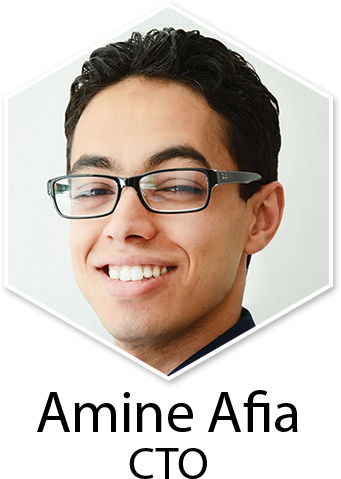
\includegraphics[width=0.20\textwidth]{amine.png}
%\caption{\label{fig:amine}This is a figure caption.}
\end{wrapfigure} 
\textbf{\textit{Amine Afia}} macht einen Doppelabschluss in Informatik am KIT (Deutschland) und INP Grenoble (Frankreich). Seine Begeisterung für die Informatik und das Lösen von Problemen haben ihn immer zum Annehmen neuer Herausforderungen geführt. Wenn er seine Fähigkeiten nicht in einem Hackathon unter Beweis stellt oder programmiert ist er in den Bergen oder mit dem Skateboard in der Stadt anzutreffen. Das Potenzial, unser tägliches Leben einfacher und das Autofahren umweltfreundlicher zu gestalten motivieren ihn und seine Mitarbeit bei Carbook. Er übernimmt das Technologieressort bei Carbook und ist motiviert, jeden Tag auch von den anderen Gründungsmitgliedern zu lernen. \linebreak

\begin{wrapfigure}{R}{4cm}%{0.3\textwidth}
\centering
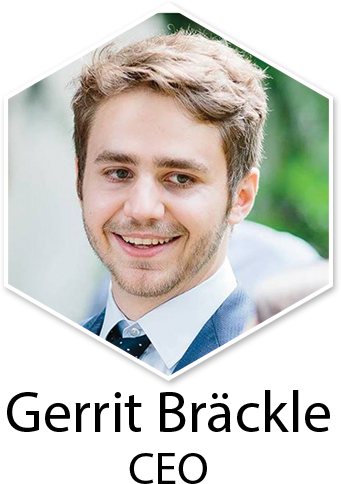
\includegraphics[width=0.20\textwidth]{gerrit.png}
%\caption{\label{fig:amine}This is a figure caption.}
\end{wrapfigure}
Geschäftsführer und Gründungsmitglied \textbf{\textit{Gerrit Bräckle}} studiert Wirtschaftsingenieurwesen am KIT im sechsten Fachsemester des Masterstudiums und hat sich in den Bereichen Service Design und Data Analytics vertieft. Mit der Gründung seines eigenen Modelabels „edd‘up“, das innovative Taschen und Kleidungsstücke mittels Upcycling aus gebrauchten Textilien herstellt, konnte er bereits erste Erfahrungen in der Startup-Szene sammeln. Zudem ist er durch ein Praktikum beim Autohersteller Mercedes Benz im Bereich Forschung und Entwicklung mit Produktentwicklungsprozessen und Projektarbeit vertraut.\linebreak

\begin{wrapfigure}{l}{4cm}%{0.3\textwidth}
\centering
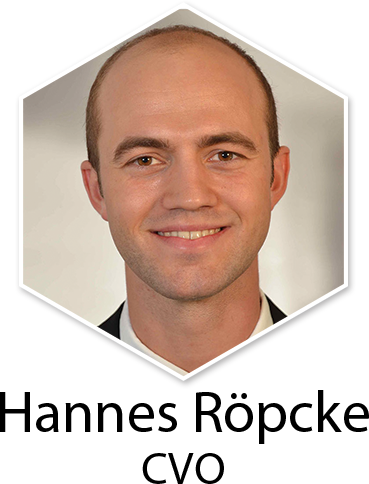
\includegraphics[width=0.20\textwidth]{hannes.png}
%\caption{\label{fig:amine}This is a figure caption.}
\end{wrapfigure}
\textbf{\textit{Hannes Röpcke}} studiert im 2. Fachsemester Master am Karlsruher Institut für Technologie (KIT). Er vertieft die Bereiche globale Produktion und Logistik sowie Fahrzeugentwicklung. Er konnte bereits Arbeitserfahrung in einem modernen, mittlerweile mittelständischen IT-Unternehmen sammeln, welches aus einem Start-Up aus dem Jahre 2010 hervorging. Dort war er unter anderem für die Finanzplanung und das Controlling zuständig. Seine Motivation liegt im Potential, das Carbook bei der heutigen Verkehrslage in Städten bietet. \linebreak

\begin{wrapfigure}{r}{4cm}%{0.3\textwidth}
\centering
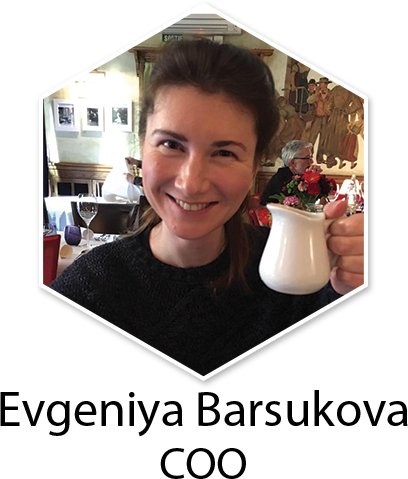
\includegraphics[width=0.20\textwidth]{jenny.png}
%\caption{\label{fig:amine}This is a figure caption.}
\end{wrapfigure}
\textbf{\textit{Evgeniya Barsukova}} studiert im 3. Fachsemester Master Wirtschaftsingenieurwesen am Karlsruher Institut für Technologie (KIT). Sie vertieft die Bereiche Virtual Engineering sowie Service Design und konnte durch ein einjähriges Arbeitsverhältnis im Global Cloud Service Center der SAP AG Erfahrungen im Projektmanagement in einem der größten Softwareunternehmen sammeln. Sie möchte gerne den Alltag leichter machen und mehr Zeit für das wichtige im Leben haben: Freunde und Familie. Deswegen glaubt sie stark an den Potential von CarBook und an alle neue Produkte , die dazu beitragen private oder geschäftliche Ziele schneller zu erreichen.  
%Hannes study the same subject as well and took the responsibility of social media for CarBook. Amine in the technical cheif officer at Carbook. \linebreak

%\begin{figure}%[ht]
    %\centering
    %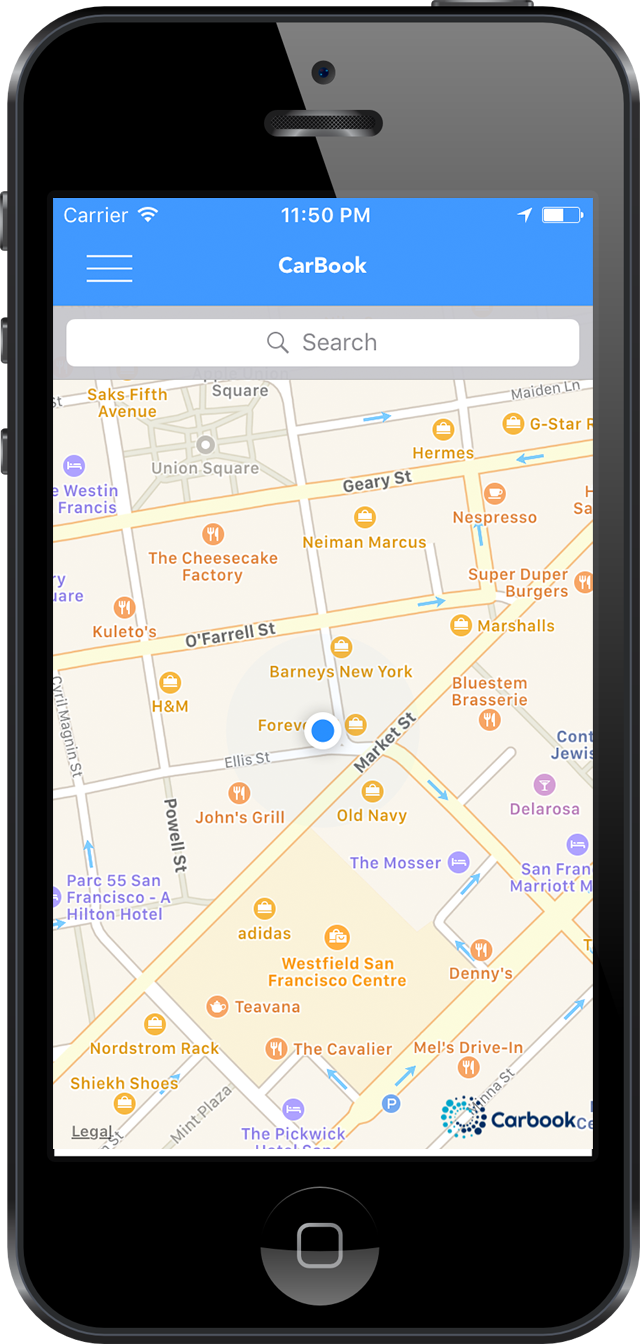
\includegraphics[width=0.3\textwidth]{home.png}
    %\begin{subfigure}{\linewidth}
    %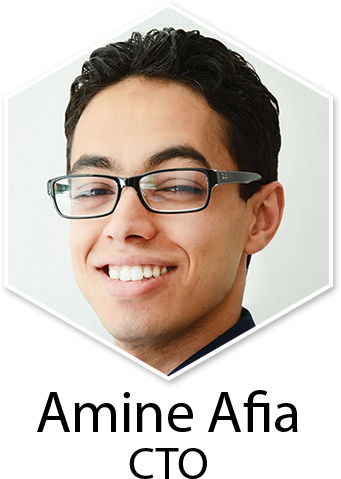
\includegraphics[width=0.15\linewidth]{amine.png}\hfill
    %\end{subfigure}\par\medskip
    %\label{fig:home1}
    
%    \begin{subfigure}{\linewidth}
%    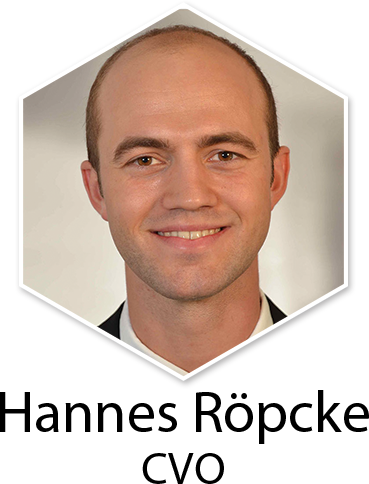
\includegraphics[width=0.15\linewidth]{hannes.png}\hfill
%    \end{subfigure}\par\medskip
%    \label{fig:home2}
%    
%    \begin{subfigure}{\linewidth}
%    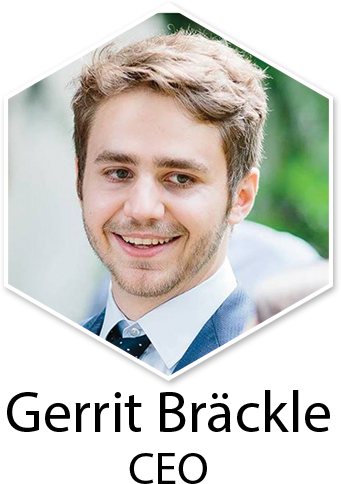
\includegraphics[width=0.15\linewidth]{gerrit.png}\hfill
%    \end{subfigure}\par\medskip
%   \label{fig:home3}
%    
%    \begin{subfigure}{\linewidth}
%    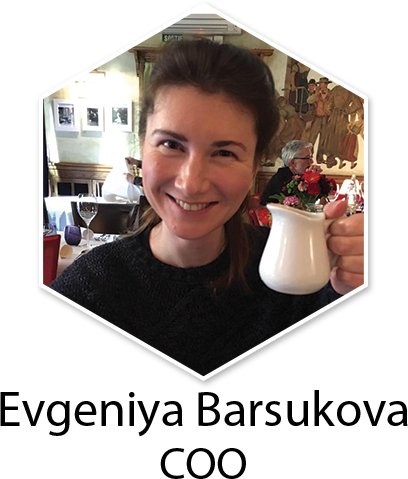
\includegraphics[width=0.15\linewidth]{jenny.png}\hfill
%    \end{subfigure}\par\medskip
%    \label{fig:home4}
%\end{figure}

\section{Innovation}
Einer der Hauptaspekte der Carbook Lösung ist die Optimierung des Parkprozesses in der Stadt mithilfe von wenig Hardware und geringem Aufwand. Zudem hilft Carbook dabei, CO2 Emissionen zu reduzieren, ungenutzte private Stellplatzkapazitäten optimal zu nutzen, sowie Zeit und Nerven der Benutzer zu schonen. Informationen über Parkhäuser und ein eigenes Nutzerprofil runden den Funktionsumfang der kostenlosen App ab. Des Weiteren soll eine Supporthotline eingerichtet werden, die bei Fragen und Problemen bei der Benutzung behilflich ist.
Die einzelnen Features der App werden im Folgenden im Detail vorgestellt. \\[55]


\begin{wrapfigure}[11]{l}{5cm}%{0.3\textwidth}
\vspace{-70pt}
\centering
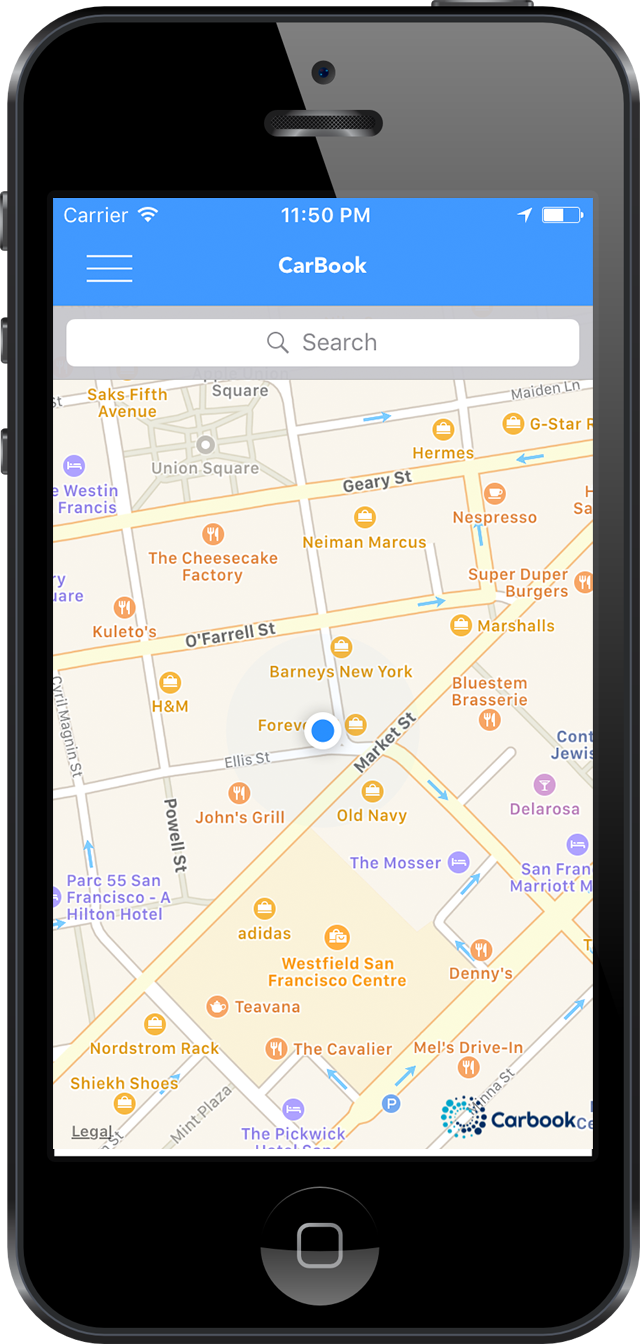
\includegraphics[width=0.3\textwidth]{home.png}
\caption{\label{fig:home} Home screen.}
\end{wrapfigure}
Der \textbf{\textit{Home}} Bereich (siehe Abbildung \ref{fig:home}) ist eine Karte, auf der Parkplatzvorschläge aus der Umgebung angezeigt werden können. Zusätzlich ist eine Suchfunktion integriert, mit der man nach Parkplätzen an einem bestimmten Ort suchen kann. Dieser Bereich ist einfach und intuitiv konzipiert, um den Nutzer beim Fahren nicht abzulenken und ihn trotzdem mit hilfreichen Informationen zu versorgen. Ein Menü-Icon oben links hilft beim Navigieren durch die App. Für zukünftige Implementierungen ist zudem ein Routenplaner auf der Karte geplant. \newpage

. \linebreak \\[20]

\begin{wrapfigure}[8]{L}{5cm}%{0.3\textwidth}
\vspace{-75pt}
\centering
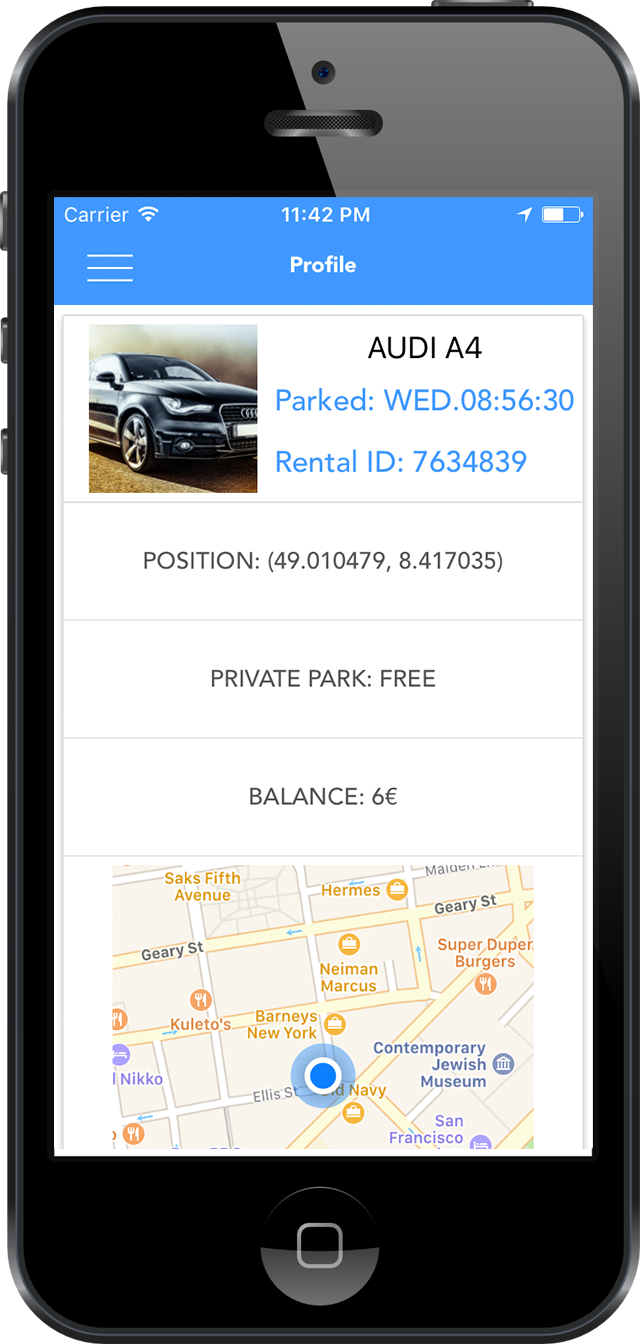
\includegraphics[width=0.3\textwidth]{park.png}
\caption{\label{fig:park} Profile screen.}
\end{wrapfigure}
Der \textbf{\textit{Auto Profil}} Bereich (siehe \ref{fig:park}) zeigt das Nutzerprofil des Fahrers und seines Autos an. Es beinhaltert Informationen über das Auto des Nutzers wie Fahrzeugmodell, Standort, Parkdauer und Guthaben (bzw. Rechnungsbetrag) für das Vermieten (bzw. Mieten) privater Stellplätze. Dieser Bereich liefert dem Nutzer volle Kostentransparenz beim Parken und hilft ihm, sein Auto in einer fremden Stadt wiederzufinden.\\ \\ \linebreak \\ \\ \\ \\ \\ \\ \\ \\ \\ \\

\begin{wrapfigure}[10]{r}{5cm}%{0.3\textwidth}
\vspace{-70pt}
\centering
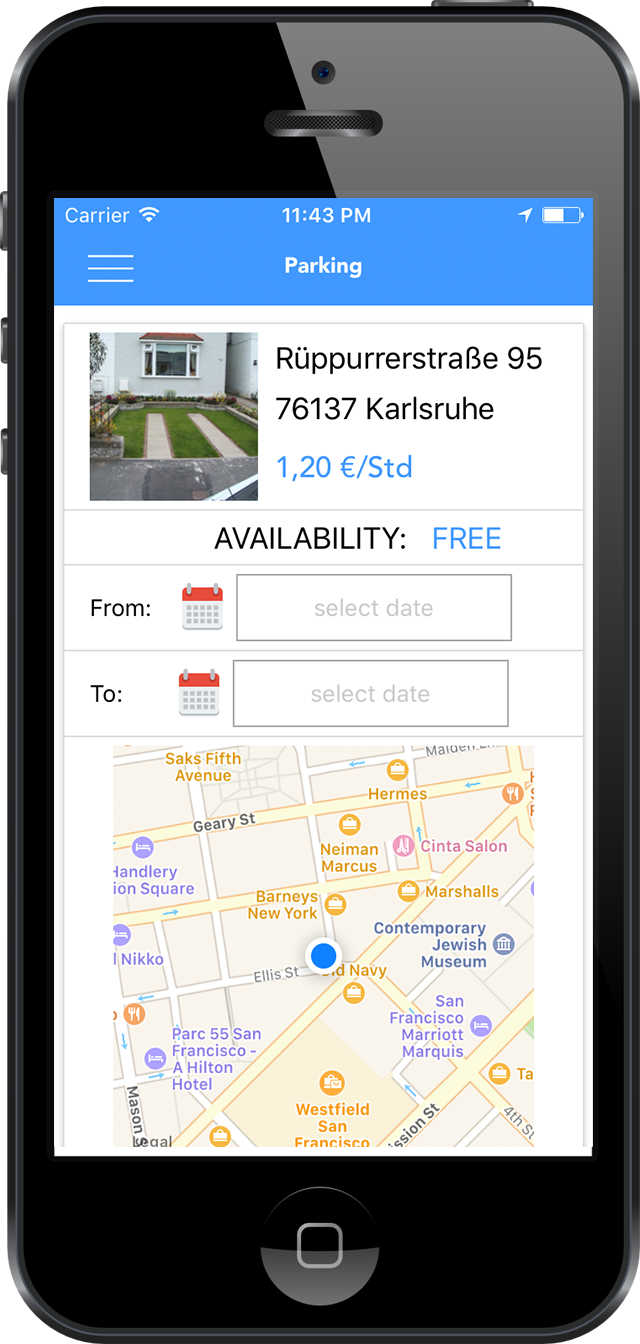
\includegraphics[width=0.3\textwidth]{rent.png}
\caption{\label{fig:miete}Rent screen.}
\end{wrapfigure}


Der \textbf{\textit{Rent}} Bereich (siehe \ref{fig:miete}) beinhaltet die Mietplattform von Carbook, auf der der Nutzer seinen privaten Stellplatz vermieten oder einen Parkplatz von einem anderen User anmieten kann. Der Nutzer kann dabei seinen eigenen Parkplatz jederzeit online stellen und der Carbook Community zur Verfügung stellen oder offline setzen, um ihn selbst zu verwenden. Bei der Anmeldung muss der Nutzer für diesen Bereich seine Kontodaten eintragen, um eine einfachen Bezahlvorgang zu gewährleisten. Diese können jederzeit in den Einstellungen geändert werden. \newpage

\section{Projektplanung (Arbeitspakete und Zukunftsaussichten)}
Unsere Projektplanung besteht aus fünf Schritten, die dazu beitragen die erste Version des Produktes zu erstellen. Zuerst planen wir die Kooperation mit Parkhäusern und Hotels und bieten das Vermieten von ungenutzten Parkflächen für daran interessierte Unternehmen. Als nächstes werden wir unser Benutzernetzwerk aufbauen, um das CarBook Grundkonzept umzusetzen und ein Smart Parking Bewusstsein bei den Nutzern zu entwickeln. Über Umfragen werden wir unsere Kunden besser kennenlernen, um die Bedürfnisse der Autofahrer zu verstehen. Basierend auf diesen Daten, kann unser Entwicklungsteam richtige Entscheidungen beim Entwurf der App treffen. Die Aufgabe der letzten Phase ist es, eine voll funktionale App zu erstellen, diese zu testen und den ersten Release in eine von uns ausgewählten Stadt,beispielweise in Karlsruhe, freizugeben. Das Diagramm in Figure \ref{fig:milestones} stellt die oben genannten Schritte im zetlichen Ablauf dar.\linebreak \\[5]

%Kooperation
%Um die Ziele unseres Geschäftsmodell zu erfüllen und einen fertigen Produkt dem Markt zu präsentieren, brauchen wir eine starke Kooperation mit Parkhäusern.
%Netzwerk
%Der zweite Arbeitspaket fängt bei der Präsenz in Sozialen Netzwerken und wird durch Aufbau effizienter Kommunikationeskanälen fortgesetzt.
%Design
%Das entworfene Allgorithmus muss passende Parkplatzvorschläge liefern. Darüber hinaus ist eine benutzerfreundliche Oberfläche ein wichtiges Punkt beim App-Entwurf.

%Implementierung
%Die Entwicklung wird unter der Berücksichtigung der State-of-the-Art-Technologien durchgeführt und am KIT getestet.
%Release
%Die erste Veröffentlichung ist erstmals für eine Stadt geplant, um das Algorithmus in der Praxis zu testen und weitere Daten zu sammeln.



%Wir fangen mit Kooperationen mit Parkhäuser als auch Hotels und alle mögliche Institute die ein Parkplatz vermieten können/wollen, dann startet der Marketing Team unsere Netzwerk zu bauen und der "Inception of Smarting Parking" Idee zu vergrößern. basiert auf diese Daten kann der Entwicklung Team richtige Entscheidungen bei der Entwurf der App treffen. Die letzte Phase ist ein voll funktionales App zu Entwickeln, testen und ein der erste Release in ein Stadt (z.B. Karlsruhe) zu Verfügung stellen. Der Diagramme im Figure \ref{fig:milestones} erklärt die verschiedene schritte in unsere Work package. \linebreak \\[5]

\begin{figure}[ht]
    \centering
    \begin{center}
      \makebox[\textwidth]{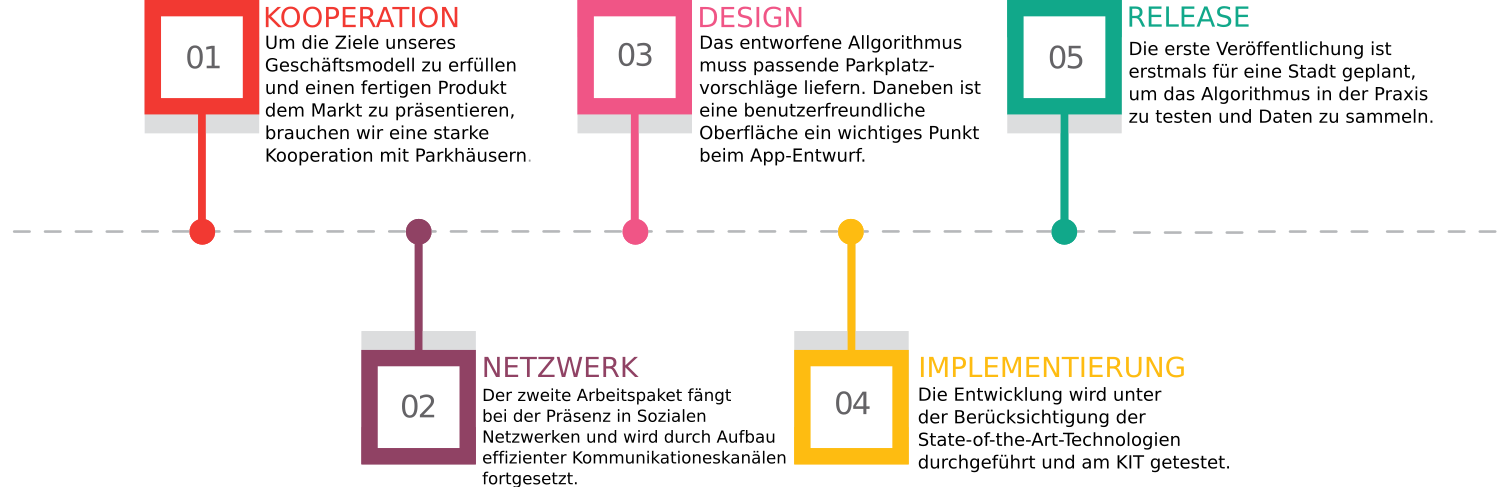
\includegraphics[width=\paperwidth]{milestones}}
    \end{center}
    
    \caption{Milestones}
    \label{fig:milestones}
\end{figure}

\\[5]
Als nächstes ist die Vergrößerung unseres Netzwerkes mit Hilfe von Marketing-Kampagnen und Freigaben in weiteren Städten geplant. Die Prognose zeigt, dass der Anteil der vernetzten Autos in 2017 um bis zu 80\% \autocite{statista7} steigt. Das kann dazu führen, dass Autohersteller die Integration der CarBook App in das Betriebssystem von Autos als lohnenswert betrachten können. Darüber hinaus wird das Recommendersystem für eine internationale Verwendung vorbereitet. Ab diesem Zeitpunkt besteht die Möglichkeit, internationale Büros zu öffnen, um CarBook App in anderen Ländern besser anzupassen. %Bei diesem Scale kommt die schritte von internationale Büros zu Öffnen, damit unsere Produkt in andere Länder richtig adoptiert kann.

%----------------------------------------------------------------------------------------
%	KAPITEL 3
%----------------------------------------------------------------------------------------

\chapterimage{headMarketing.png}
\chapter{Markt/Wettbewerb}

Da der Erfolg unseres Produktes sehr stark von der Nutzerzahl abhängt, haben wir uns eine Vorgehensweise für einen erfolgreichen Markteintritt überlegt, die unser Produkt dabei unterstützt beim Kunden schnell anzukommen. Unsere Markteintrittsstrategie beinhaltet drei Aspekte. Zuerst haben wir die aktuelle Marktsituation analysiert und dann die existierenden Wettbewerbersprodukte angeschaut, um identifizieren zu können, was wir an unserem Produkt besser machen können im Vergleich zu den Wettbewerbern und welche Taktiken wir vermeiden sollen, um kompetitiv zu bleiben. Zum Schluss haben wir nach potentiellen  Kooperationspartnern gesucht, um unseres Produkt für den Kunden attraktiver und funktionsreicher zu machen. Ausserdem haben wir uns mit dem App Präsenz Konzept auseinandergesetzt und sind Schritt für Schritt die Expertenempfehlungen \autocite{softwaresupply} gefolgt, um unsere Zielgruppe zu erreichen. \\ \\
Unsere Marktanalyse unterstützen wir durch eine selbst ausgearbeitete und durchgeführte Umfrage sowie durch offizielle Statistiken zum Thema Parking.\\ \\
In diesem Kapitel schildern wir die aktuelle Marktanalyse für die Automobilbranche, präsentieren unsere Ergebnisse der Umfrage, vergleichen unsere App mit den Konkurrenten und stellen unsere Herangehensweise für die Produkteinführung im App Store dar.

\section{Marktanalyse des Automotive Marktes und dessen Einfluss auf das Strassenverkehr} 

Weltweit fahren 1,2 Milliarden Fahrzeuge \autocite{greencarreports}. Der Fahrzeugbestand in Deutschland laut Statista beträgt 53 Millionen \autocite{statista1}, davon 45 Mio. Personenkraftwagen \autocite{statista2} (Pkw). Autofahrer sind durchschnittlich 560 Millionen Stunden auf der Parkplatzsuche unterwegs\autocite{welt1}. 30 \% des Strassenverkehrs entsteht durch die Suche nach einem Parkplatz\autocite{apcoa, forbes}. Das Parken verursacht gravierende Folgen, wie es in der Abbildung 1 zu sehen ist. Mit der CarBook App wollen wir stressige Situationen auf den Strassen vermindern und Mehrwert für unseren Kunden schaffen. \\ \\
Wir entwickeln eine App für die Autofahrer und dementsprechend haben wir uns erkundigt, wie Autos in der Zukunft ausgestattet werden, ohne dabei den gegenwärtigen Fahrzeugbestand zu vernachlässigen. Dadurch dass es immer mehr Connected Autos (ein Auto mit Internetzugang und/oder externer Vernetzung) in den nächsten Jahren auf den deutschen Markt kommt, wird die Verbreitung unserer App dementsprechend zunehmen. Seit diesem Jahr besteht die Möglichkeit in einigen Fahrzeugen leicht per vorhandenen USB- Kabel einen iPhone oder Android Smartphone an das Infotainment System anzuschliessen und die darauf befindlichen Applikationen auf dem Display zu sehen und zu nutzen, wie man auf dem Bild \ref{fig:carplayandandroidauto} sieht. Im vergangenen Jahr waren es weltweit  2,56 Mio. Autos mit Apple CarPlay und Android Auto unterwegs und es sollen fast 200 Mio. kompatible Pkw  bis 2020 werden \autocite{welt2}. Für uns bedeutet es, dass unsere Kunden Carbook App einfach auf dem Display von ihrem Auto und nicht nur vom Handy nutzen können, was die Handhabung schneller und leichter macht. Was die „alten“ Fahrzeuge betrifft, bieten wir unseren Autofahrern eine günstige Plug-n-Play GPS Lösung zum Einsatz, um ein Auto lokalisieren zu können, damit unsere Kunden die Funktionen unserer App im vollen Umfang nutzen können. \\ \\
\linebreak
\begin{figure}[ht]
    \centering
    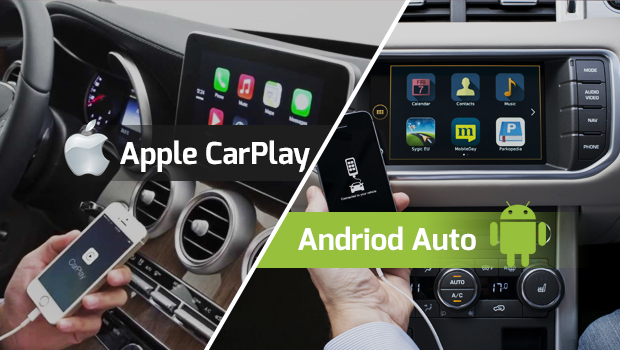
\includegraphics[width=0.8\textwidth]{carplayandandroidauto}
    \caption{Apple CarPlay und Android Auto}
    \label{fig:carplayandandroidauto}
\end{figure} \linebreak
Unsere Kunden für CarBook App sind primär die Autofahrer, es lässt sich jedoch auf Kooperationspartner erweitern, auf die wir im Kapitel 3.4 mehr eingehen.\\ \\
Das Marktvolumen bezieht sich auf die Anzahl an Autofahrer in Deutschland. Dies beträgt in Jahr 2016 39,31 Mio.\autocite{statista3}.
Um unsere App mit praktischen Funktionalitäten auszustatten, haben wir eine Umfrage \autocite{umfrage} durchgeführt. \\ \\
Die Umfrage umfasste 14 Fragen, von denen einige aus Ja/Nein Fragen, wie z.B. „Wissen Sie eine App, die die Informationen über Parken oder Payment liefert?“, einige aus Entscheidungsfragen, bei denen aus zwei oder mehreren Auswahlmöglichkeiten nur eine ausgewählt werden konnte, oder Entscheidungsfragen mit mehreren Auswahlmöglichkeiten, wie beispielsweise „Welche Art der Information würden Sie gerne in einer Parking App haben wollen?“.  Paar Fragen könnte man als Umfrageteilnehmer selbst mit eigenem Text ausfüllen, z.B. „Welche Art der Information würden Sie gerne in einer Parking App noch haben?“. Die Umfrage war eine Woche lang im World Wide Web freigeschaltet. Wir haben 32 Antworten bekommen, aus denen wir unsere Schlussfolgerungen für die Weiterentwicklung unserer App schliessen konnten. Wir fanden interessant die Tatsache, dass nur 9,4 \% der Befragten wussten über Existenz von Parkplatz-Apps und keiner von unseren Befragten hat jemals eine App für das Parken benutzt.  Deswegen werden wir unsere Präsenz auf dem Markt durch Social Network Plattformen, wie Twitter, Facebook und Instagram stärken.  Auf YouTube werden wir unsere Videos für die Benutzung der App sowie für die Installation der Plag-n-Play GPS Systems zu Verfügung stellen. Durch Außenwerbung, z.B. an den Haltestellen sowie mit Hilfe von Print Medien werden wir uns bekannt machen. Obwohl keiner der Befragten jemals eine Parpklatz-App benutzt hat, würden 84,4 \% gerne diese benutzen und 62,5 \% würden gerne einen privaten Parkplatz mieten als in einem Parkhaus oder in den öffentlichen Stellplätzen parken. Folgende 3 Punkte sind für unsere Kunden am wichtigsten, je nach Priorität: Zahlungskonditionen (84,4 \%), Interaktives Parkleitsystem (81,3 \%) und „4 Parkplätzen werden innerhalb der nächsten 10 Minuten frei“(71,9 \%). Und für 6,3 \% reicht die Abbildung von Parkplätzen auf der Karte ohne zusätzliche Information. Wir werden noch weitere Umfragen durchführen, um CarBook möglichst angepasst an Bedürfnisse unserer Kunden zu entwicklen. Da unsere App die Fahrsituation auf den Strassen verbessern soll, werden wir versuchen Kooperationspartner anzulocken.

\section{Alleinstellungsmerkmal und Kundennutzen}

Laut Statistiken würden 53 \% \autocite{statista4} der Autofahrer ein System nutzen, die auf die aktuell verfügbaren Parkplätze verweist, wenn es kostenlos wäre. \\ \\
Mit CarBook möchten wir Parkplatzangebotsübergreifend auf dem Markt agieren. Schon in der kostenlosen Version kann der Autofahrer nach allen möglichen Arten von Parkplätzen (öffentliche Stellplätze, Parkhäuser, private Parkplätze, kostenlos und kostenpflichtig) suchen und diese auch per App bezahlen können. Bezahlen kann man mittels Android oder Apple Pay, PayPal oder EC-Karte. Wir profitieren von jedem dem unsere App gefällt und der unsere App nutzt. Durch Weiterempfehlungen kreieren wir einen Netzwerk von Autofahrer/Nutzer, die ihrerseits einen Netzwerk von Parkplätzen generieren. Unser selbstlernendes Algorithmus bringt den Mehrwert für unsere Kunden, dadurch das es nicht eingetragene Stellplätze als solche erkennt und automatisch in das Datenbank einträgt. Stellplätze und Parkhäuser  werden von uns in das Datenbank eingetragen. Wir versichern unsere Kunden, dass  auf der Karte nur vertrauenswürdige Informationen über die Parkplätzen gezeigt werden. In Echtheit wird die Besetzung eingezeigt. Die Parkleitsystem - Anzeigetafeln, die wir von dem Stadtverkehr kennen, die Autofahrt zu einem freien Parkplatz leiten soll - werden wir auf unsere Karte abbilden. Hinzu kommt eine Funktion der Freigäbe der von einem Autofahrer besetzten Parklücke, die er innerhalb von den nächsten 10 Minuten verlässt. Der Autofahrer kann den passenden Stellplatz online buchen, wenn der Parkplatz dies erlaubt, z.B. wenn es sich um einem Parkhaus handelt. CarBook kann zu Ihrem ausgewähltem Parkplatz navigieren und verfügt über eine Funktion, die Ihr Auto wiederfindet, falls Sie es vergessen haben, wo Sie Ihr Auto geparkt haben. Mit CarBook sparen Sie Ihr Zeit und Geld und das Parken wird leicht und stressfrei ohne unnützlichen Hin- und Herfahren durch die Stadt. 
\section{Wettbewerber}
Für eine bessere Einschätzung des Produkterfolges haben wir eine Wettbewerbsanalyse der auf dem deutschen Markt verfügbaren Parkplatz-Apps durchgeführt. Es gibt schon viele Apps, die die Parksuche unterstützen. Sie unterscheiden sich zwar in ihren Einsatzmöglichkeiten: Parkplatz im Parkhaus oder offener Stellplatz oder Mietplattform für Privaten Parkplätzen und richten sich an unterschiedliche Zielgruppen: Parkplätze für alle oder Behindertenparkplätze, kostenpflichtige und kostenlose.\\ \\ 
Sehr viele Apps begrenzen ihre Benutzergruppe von Anfang an in dem sie z.B. nur für eine Betriebssystem entwickeln, wie wir in der Abbildung so und so sehen, die App kann durchaus gut sein, aber nicht alle Autofahrer können es benutzen. Einige Apps haben schon an ihrer Existenz gescheitert, wie z.B. Park2gether, die eine Sharing-Plattform für private Parkplätze konzipiert wurde. Man findet zwar die Informationen und Bewertungen über Park2gether, aber sie ist in keinem App Store zu finden.\\ \\
Wir haben einige Apps, die aus unserer Sicht interessant werden können ausgesucht und mit unserer App verglichen. Es gibt noch keine App, die alle Funktionalitäten abdeckt. Bezahlung wird nur von Parkopedia angeboten, wir haben diese Funktion aber in der App nicht gefunden. Vermutlich ist sie unter der Premium Version versteckt, wobei es keinerlei Informationen weder in der App noch auf der Homepage über die Vorteile durch das Upgraden auf Premium gibt. Parking Slot App positioniert sich als eine kostenlose App für die Suche nach kostenlosen und Behindertenparkplätzen. Bei der Eingabe des Ortes werden Parkplätze auf der Karte angezeigt und mittels Filter kann man die Parkplätze nach ihrer Kategorie (Alle, Behindertenparkplatz, Kostenfrei, Zeitweise Kostenfrei) sortieren.  Ohne Sortierung zeigt uns die Karte die verfügbaren Parkplätzen in Karlsruhe. Als wir nur behinderten Parkplätze angezeigt haben wollten, wurden uns in Karlsruhe keine Parkmöglichkeiten angezeigt. Wenn man nach kostenlosen Parkplätzen filtert, werden nur noch zwei angezeigt. Die App ist nicht vertrauenswürdig, da z.B. die Parkplätze am KIT Campus werden auch als frei verfügbare Plätze angezeigt, wobei diese Parkplätze nur für die Mitarbeiter von KIT gedacht sind.\\ \\
\begin{figure}[ht]
    \centering
    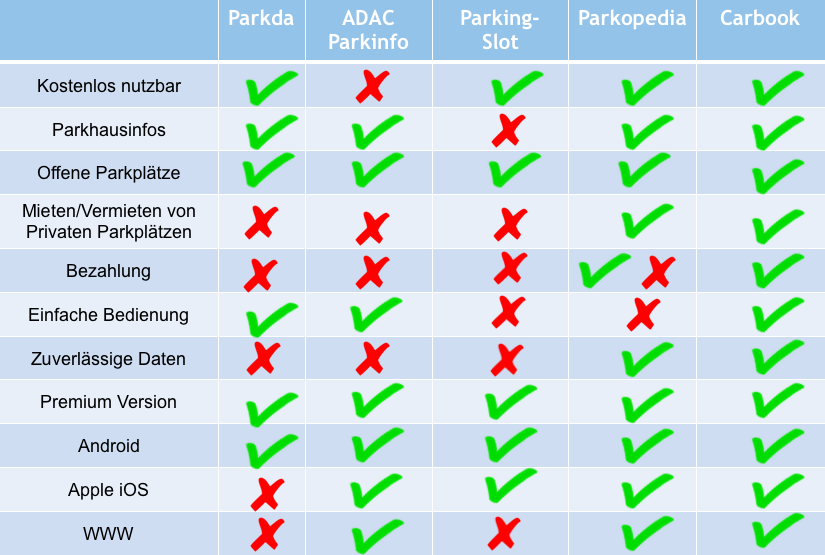
\includegraphics[width=0.9\textwidth]{Wettbewerber}
    \caption{Vergleich aktueller Wettbewerber}
    \label{fig:Wettbewerber}
\end{figure} \\
Parkopedia ist im großen und ganzen eine ganz gute App, aber die gebaute Funktionen sind nicht selbsterklärend und die Funktion „Buchen“ von Parkplätzen, die auf der Parkopedia Webseite verfügbar ist, ist in der App nicht zu finden. Und wie schon vorher erwähnt, es gibt keine Beschreibung von der Premium Version. ADAC Parkinfo steht für die Autofahrer für \EUR{1,99} zum Downloaden und verfügt laut Rezessionen über gar keine Parkplätze in Berlin, zeigt falsche Informationen über die Kosten und Besetzung von Parkhäusern\autocite{googleplay}. Weitere Unterschiede zu unserem Produkt sind der Tabelle \ref{fig:Wettbewerber} zu entnehmen.


\section{Markteintritt}
Unser Ziel ist es, den Markt-eintritt von einer Seite möglichst schnell durchzuführen und von der anderen Seite möglichst realistisch zu gestalten. \\ \\
Für eine App ist es eine gute Platzierung im App Store sehr wichtig, weil es schnellere Verbreitung des Produktes sichern kann. Um in die Top 10 der besten Apps zu kommen, müssen wir eine Benutzeranzahl von 16500 zu erreichen\autocite{statista5}. Deswegen folgen wir den Empfehlungen der App-Experten und haben uns erstmal ein gutes App Titel und Logo überlegt. Carbook Titel und Icon steht für die Netzwerke für Autofahrer und/oder Autobesitzer, sie ist ansprechend und verkörpert die eigentliche Funktionen des Produktes - Netzwerk von Autos. Wir setzten auf unser blaues App Logo, das das Aufmerksamkeit auf sich lenkt. In 34 \% der  Downloads haben Apps, die sich mit Nachrichten, Tipps und Tricks beschäftigen, eine blau Farbe\autocite{iphonetricks}.  Der Autofahrer möchte leicht und schnell ans Fahrtziel ankommen und hat eine bestimmte Vorstellung, wie eine gute App aussehen soll. Deswegen legen wir uns sehr viel Wert auf die Auswahl von Bildern, die auf den ersten Blick die wichtigsten Funktionalitäten in der App Beschreibung darstellen. Wir bitten unseren Kunden eine kostenlose App, was auch, wie schon vorhin erwähnt, attraktiv für den Nutzer ist. Die App wird im Google und Apple App Stores verfügbar. Die Carbook Webseite kann man einfach auf dem Laptop oder Tablet über einen Webbrowser abrufen und unsere App herunterladen sowie das \emph{GPS} Tracking Gerät bestellen.\\ \\
Wir werden in allen deutschen Klein- und Großstädten präsent. Mit Google Earth und Google Street View schaffen wir uns die Informationen über offenen Parkmöglichkeiten am Straßenrand und werden erstmals selbst in den Städten, wie z.B. Karlsruhe, fahren und diese prüfen sowie andere Leute, unsere Bekannten und Freunde in anderen Städten engagieren dies zu machen.  Dadurch werden wir das Bestehen der Parkplätze sicherstellen. Die Information über verfügbare Parkhäuser sind auf der Webseiten deutscher Städte und Kommunen abrufbar. Unsere Premium Version schaltet die Bannerwerbung ab. \\ \\
Wir möchten mit dem größten Verkehrsklub \emph{ADAC} kooperieren und mit dem monatlichen ADAC Magazin Carbook allen Mitgliedern als Standard Produkt für Parkplatzsuche anbieten. Wir planen eine Kooperation mit den Parkhäusern, zuerst werden wir versuchen die kleinen, wie z.B. Parkhaus von einem Einkaufszentrum und dann die größten Parkhausbetreiber wie APCOA und Q-Park \autocite{statista6} zu gewinnen. Wir möchten auch mit den Städten kooperieren, die auch über aktuellen Informationen der Belegung von Parkhäusern in deren Region verfügen, sowie über die offenen Stellplätzen. Hotels und Unternehmen verfügen auch über sehr viele Parkplätze, die einfach leer stehen, die aber durch CarBook vermittelt werden könnten. Mit unserem Produkt können sie ihre freistehende Parkplätze unseren Kunden anbieten.  Dafür brauchen wir ein klare Vorstellung dafür, wie wir unsere Partner gewinnen und einen strukturierten Finanzplanung.


%----------------------------------------------------------------------------------------
%	CHAPTER 4
%----------------------------------------------------------------------------------------

\chapterimage{headPlanung.png} % Chapter heading image
\chapter{Unternehmensplanung}
In der Unternehmensplanung wird zwischen operativer, taktischer und strategischer Planung unterschieden. Um die in einem jungen Unternehmen existierenden dynamischen Arbeits-, Finanz- und Organisationsprozesse zu stabilisieren, müssen diese schon frühzeitig geplant und als stabile Kernprozesse etabliert werden\autocite{koll}.\\ \\
Bei Carbook handelt es sich um ein E-Start-Up, das in der Net Economy gegründet werden soll. Die Erfolgsfaktoren hierfür lassen sich in die fünf Bereiche Management, Marktzugang & Marketingplanung, Produkt & Service, Finanzen sowie Prozesse bzw. Unternehmensorganisation gliedern\autocite{koll,mcdo}. In unserem Management kommen aufgrund unserer unterschiedlichen Studienschwerpunkte, verschiedene technische, soziale und methodische Fähigkeiten zusammen, um die verschiedenen Herausforderungen, denen ein Start-Up gerade in den ersten zwei Jahren ausgesetzt ist, entgegenzutreten.
Unseren Marktzugang sichern wir uns durch die Lösung eines in nahezu allen Städten anzutreffendes Problem unserer Kunden: Die begrenzte Verfügbarkeit von Parkplätzen und die damit verbundene Parkplatzsuche. Um das hierfür notwendige Netzwerk zu etablieren und möglichst viele Nutzer zu erreichen, wollen wir eng mit Parkausbetreibern und der Stadtverwaltung der jeweiligen Städte zusammenarbeiten. \\ \\
Unser Produkt ist eine Weiterentwicklung und Fusionierung bestehender Technologien. Durch die Kombination von Parkplatzempfehlungssystem inklusive Parkhäusern und ausgewiesenen Parkplätzen der Stadt, E-Payment-System und weiteren Funktionen wie: Diebstahlschutz, Vor-Ort-Empfehlungen etc., stellen wir dem Nutzer eine innovative App zur Verfügung, die dem Nutzer einen echten Mehrwert einbringt. \\ \\
Im folgenden Kapitel werden die Marketingplanung, die Finanzplanung sowie die Unternehmensorganisation in den ersten zwei Jahren des Carbook-Start-Ups ausführlicher behandelt.

\section{Finanzplanung} 
Bei einem Start-Up sind für die Finanzplanung vier Grundsätze von Bedeutung: Profitabilität, Liquidität, Effizienz und Stabilität\autocite{barr}. Wichtig hierbei ist es, den Investoren Klarheit und Transparenz über die aktuelle und zukünftige, geplante Finanzlage des Start-Ups zu schaffen. Dazu zeigen wir wie hoch die finanziell benötigten Mittel sein werden und unter welchen Bedingungen Carbook erfolgreich auf den Markt gebracht werden kann.

\subsection{Preismodell und Einnahmenquellen}
Die erste Version von Carbook wird als Free- und als Premium-App angeboten, die von jedem Nutzer in den genannten Stores heruntergeladen ohne Einschränkungen verwendet werden kann.
Dabei ist geplant in die Free-App Werbebanner, die in der Benutzeroberfläche individuell geschaltet werden können, zu integrieren und Werbepartnern als attraktive Werbeflächen zur Verfügung zu stellen. Zudem können sich Werbepartner Vor-Ort-Empfehlungen zu Werbezwecken reservieren. Durch diese Werbemöglichkeiten lässt sich bereits ein Teil der App finanzieren.
Eine weitere Einnahmequelle stellt die Zahlungsabwicklung durch E-Payment-Dienste dar. Bei jeder Parkplatzreservierung wird die Bezahlung über einen solchen Dienst abgewickelt, wobei unserem Unternehmen ein Teil jeder Transaktion gutgeschrieben wird.
Die dritte Einnahmequelle ist unsere modifizierte Smart-Box, die von uns mit der notwendigen Software ausgestattet und von Carbook als Zwischenhändler vertrieben werden soll.
\subsection{Finanzplan}
Der Finanzplan von Carbook für die nächsten zwei Jahre ist ein zentraler Bestandteil unseres Business-Plans. Der Kapitalbedarf aus Fremdfinanzierung sinkt dabei in Abhängigkeit des Entwicklungsstandes unseres Start-Ups. Nachfolgend werden alle Meilensteine mit den dazu anfallenden Kosten näher beschrieben. \\ \\
In den ersten drei bis sechs Monaten werden für Entwicklung und Desing einer nahezu marktreifen App vor allem Personalkosten für Entwickler anfallen. Dabei zahlen wir jedem Gründer einen kalkulatorischen Lohn von \EUR{1000} aus, der laut Exist-Gründerstipendium zur Sicherung des persönlichen Lebensunterhalts dienen soll\autocite{existlohn}. Insgesamt wollen wir ein Team von sieben Mitarbeitern bilden, von denen inklusive des Gründers Amine Aifia vier als Entwickler arbeiten. Somit fallen jeden Monat \EUR{3000} an zusätzlichen Personalkosten an. Die größe des Entwicklerteams wird nach der Entwicklungsphase reduziert. Nach der Markteinführung wird das Team um Marketingmitarbeiter ergänzt.\\ \\
Ab dem sechsten Monat werden die Kosten für das Serverhosting steigen, da ab diesem Zeitpunkt unsere Datenbank mit den bereits verfügbaren Daten der Stadtverwaltung und den städtischen Parkhäusern erweitert und gesichert werden und in Quartal 3 \& 4 die Anzahl der Testnutzer für einen realen Testbetrieb erhöht werden sollen.\\ \\
Nach zwölf Monaten wollen wir eine marktreife App auf den Markt bringen. Ab diesem Zeitpunkt werden die Marketingkosten für Werbung auf den Social-Media-Plattformen, Printmedien und anderen Kommunikationskanälen steigen. Zudem wollen wir auf Innovationsforen und IT-Messen Präsenz zeigen, wofür wir ein Reisebudget von \EUR{500}/Monat sowie Materialkosten (Rollups, Banner, Flyer, Business Cards etc.) von einmalig \EUR{500} benötigen. Die Entwicklungskosten hingegen sinken.\\ \\
Bis zum 18. Monat soll die Carbook Community auf über 100.000 Nutzer anwachsen. Dafür werden leistungsstarke und sichere Cloud-Server benötigt, was die Kosten für das Serverhosting weiter steigen lässt. Die Hostingkosten für das erste Jahr liegen somit bei etwa \EUR{1200} und verdoppeln sich im zweiten Jahr auf \EUR{2400}.
Da wir in den ersten drei bis sechs Monaten planen, ein größeres Entwicklerteam zusammenzustellen, sehen wir eine Bürogröße von ca. 50-70 qm vor. Im Raum Karlsruhe ergibt sich für diese Größe, inklusive Mobiliar, ein Mietpreis von ca. \EUR{600}/Monat. Zusätzlich entstehen Kosten für Laptops und Drucker von einmalig \EUR{4500}. Sie werden als Aufwand für Abschreibungen verbucht. Für die Internet- & Telefonverträge fallen jedes Jahr \EUR{150} an. Alle Aufwendungen sind in Tabelle \ref{fig:Aufwendungen} aufgeführt.\\ \\
Unsere App soll, wie bereits erwähnt, als Free- und als Premium-Version zur Verfügung stehen. Die Premium-Version wird mit \EUR{1,99} bepreist. Dabei rechnen wir in den ersten sechs Monaten mit 2000 Downloads der Premium-Version. 
Die Free-Version hingegen wird durch im heutigen Performance Marketing übliche Abrechnungsmethoden finanziert\autocite{abrechnungsmodelle}. Zu den gängisten Methoden gehört das CPM-Modell (cost-per-mille), in dem der Werbepartner einen Preis pro 1000 Aufrufe einer bestimmten Seite zahlt\autocite{adsense,mobilgeld}. Für unsere Carbook-Plattform fordern für den Faktor CPM einen Betrag von \EUR{0,29} von den Werbepartnern. Ein weiteres Modell ist das CPC-Modell (cost-per-click), wobei ab einer gewissen Anzahl an Clicks auf ein Werbebanner vom Werbepartner ein Preis bezahlt wird. Für Carbook setzen wir den Preis für den Faktor CPC auf \EUR{0,49}. Die CTR (click-through-rate) liegt in Deutschland bei ca 0,1\%\autocite{ctr}. Bei potentiellen 98000 Nutzern der Free-Version in Deutschland werden somit in den ersten sechs Monaten ab der Markteinführung bei 25000 Nutzern, die Carbook täglich verwenden, und durchschnittlichen 10 Aufrufen der Seite pro Nutzer, pro Tag, etwa \EUR{72} an Werbeeinnahmen durch das CPM-Modell erzielt. Die Werbeeinnahmen des CPC-Modells sind zu diesem Zeitpunkt noch zu gering um in die Berechnung mit aufgenommen zu werden.\\ \\
\begin{figure}
    \centering
    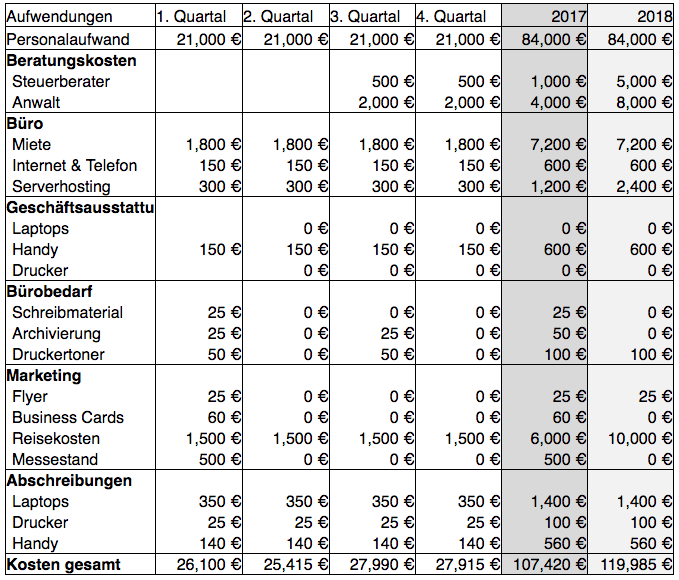
\includegraphics[width=0.9\textwidth]{Aufwendungen}
    \caption{Aufwendungen Q1-Q8}
    \label{fig:Aufwendungen}
\end{figure}
Möchte ein Parkplatzbesitzer (z.B. Privatpersonen oder Firmen) seinen Parkplatz anbieten, so nennt er uns seinen gewünschten Preis. Wird dieser Parkplatz von einem Autofahrer angefordert, so berechnen wir zum geforderten Mietpreis eine Servicegebühr von 15\%. Der Parkplatzbesitzer bekommt so seinen gewünschten Betrag von uns ausgezahlt. Bei einem angenommenen durchschnittlichen geforderten Parkpreis von etwa \EUR{2} entspricht die Provision somit 30 ct. Der Mieter muss für den Parkplatz somit \EUR{2,30} bezahlen.\\ \\
Für die Vermittlungen von Parkplätzen in Parkhäusern verlangen wir vom Parkhausbetreiber eine Provision von 10\% des Gesamtbetrages. 
Zusätzlich können Firmen ihre, meistens am Wochenende freistehende,  Parktflächen durch uns vermitteln lassen und somit eine zusätzliche Einnahmequelle generieren.\\
\begin{figure}[ht]
    \centering
    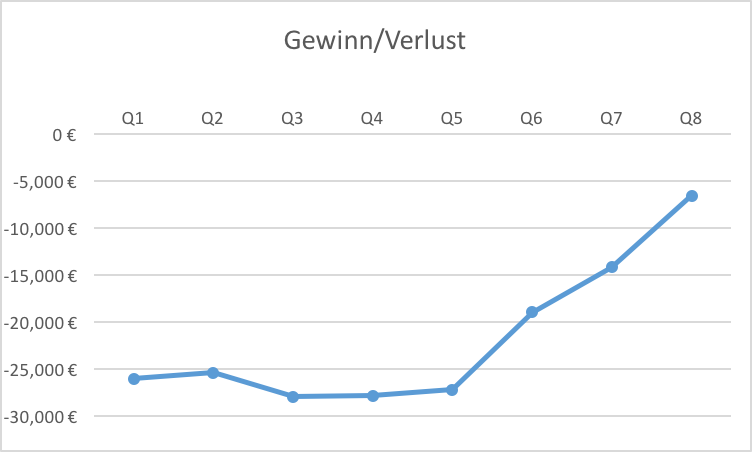
\includegraphics[width=0.9\textwidth]{GuV}
    \caption{Gewinn- und Verlustkurve Q1-Q8}
    \label{fig:GuV}
\end{figure} \\
Eine weitere Möglichkeit mit Carbook Geld zu verdienen besteht darin, dass sich Werbepartner wie Restaurants Vor-Ort-Empfehlungen reservieren können. Sie werden dann in der Carbook-Map als POI (point-of-interest) angezeigt oder in unserer App durch ein pop-up dargestellt.\\
Die Smart-Box wird planmäßig jedoch erst später eingeführt und ist deshalb noch nicht im Finanzplan für die ersten zwei Jahre enthalten. Der Einkaufspreis eines solchen Moduls liegt bei etwa \EUR{10} und wird von uns mit \EUR{11,99} bepreist.
Die geplanten Ausgaben und Einnahmen spiegeln sich in der folgenden Gewinn- und Verlustkurve \ref{fig:GuV} wider.\\
\begin{figure}[ht]
    \centering
    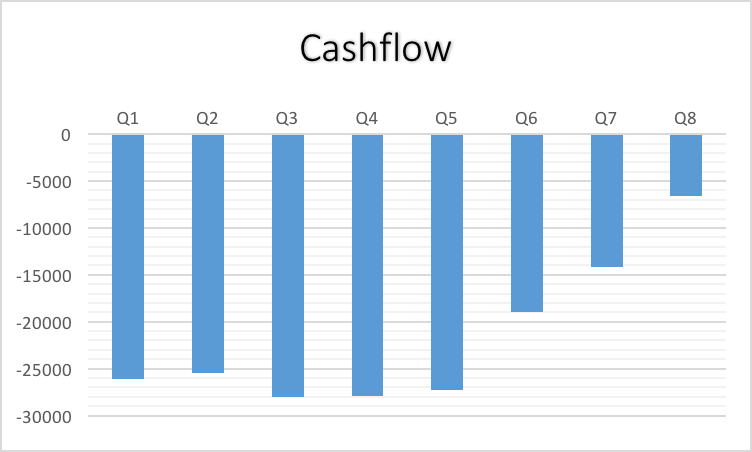
\includegraphics[width=0.9\textwidth]{Cashflow}
    \caption{Cashflow Q1-Q8}
    \label{fig:Cashflow}
\end{figure}\\ 
Wie in \ref{fig:GuV} zu erkennen ist, fallen besonders in den Quartalen 1-4 erhebliche Kosten an. Ab Q5 werden wir in der Lage sein, die Kosten durch stetig steigende Werbeeinnahmen und eine Erhöhung der Bezahlvorgänge mehr und mehr zu decken. In \ref{fig:Cashflow} ist der Cashflow für die ersten beiden Geschäftsjahre aufgeführt. Es ergibt sich ein Kapitalbedarf von etwa \EUR{175000}, der zum Teil durch das Exist-Stipendium finanziert werden soll. Zudem wollen weitere Firmen als Investoren dazu gewinnen.\newpage

\section {Unternehmensorganisation}
\subsection{Rechtsform}
Bei der Überlegung einer geeigneten Rechtsform für ein Start-Up beschränkt sich die Auswahl aufgrund des zumeist geringen Startkapitals auf eine Unternehmergesellschaft (haftungsbeschränkt) (UG) oder eine offene Handelsgesellschaft (OHG).\\ \\
Die OHG wird nach deutschem Recht von zwei oder mehr natürlichen oder juristischen Personen gegründet. Die Gründung ist nicht an ein bestimmtes Mindestkapital gebunden. Außerdem ist sie in gewisser Weise rechtsfähig (obwohl sie keine juristische Person ist).  Zu beachten ist allerdings, dass die einzelnen Gesellschafter neben dem Gesellschaftskapital auch mit ihrem Privatvermögen voll haften \autocite{handelsgesellschaft} 
Eine UG (haftungsbeschränkt) kann als Vorform einer Gesellschaft mit beschränkter Haftung (GmbH) angesehen werden. Sie zeichnet sich dadurch aus, dass lediglich ein Startkapital von \EUR{1} zur Gründung benötigt wird. Von den erwirtschafteten Gewinnen werden jährlich 25\ dem Stammkapital zugeführt, bis das Mindestkapital für die Gründung einer GmbH ( \EUR{25.000}) erreicht ist. Da die UG rechtlich wie eine GmbH zu betrachten ist, entfällt die Haftung mit dem Privatvermögen durch die Gesellschafter %(https://de.wikipedia.org/wiki/Unternehmergesellschaft_(haftungsbeschr%C3%A4nkt)). 
Aufgrund des geringen Startkapitals sowie des geringeren Haftungsrisikos gegenüber der OHG hat sich die UG (haftungsbeschränkt) als Rechtsform in der Gründerszene etabliert.\\ \\
Für die Gründung von Carbook bietet sich aufgrund dieser Vorteile die Rechtsform der UG (haftungsbeschränkt) an. Mit einer Einlage von \EUR{500} durch jedes Gründungsmitglied ergibt sich daraus ein Startkapital von \EUR{2.000}.

\subsection{Organisation}
Aufgrund der überschaubaren Aufgabenbereiche und homogenen Produktlinie von Carbook wird zu Beginn eine funktionale Organisationsstruktur gewählt. Diese ist besonders für kleine und mittlere Betriebe interessant, da sie sich durch eine klare Aufgabenverteilung und abgegrenzte Kompetenzbereiche auszeichnet. Für Carbook ergibt sich daraus eine Gliederung in die Bereiche Geschäftsführung, Softwareentwicklung, Marketing/Sales und Finanzen/Recht. \\ \\

\begin{figure}[ht]
    \centering
    \centerline{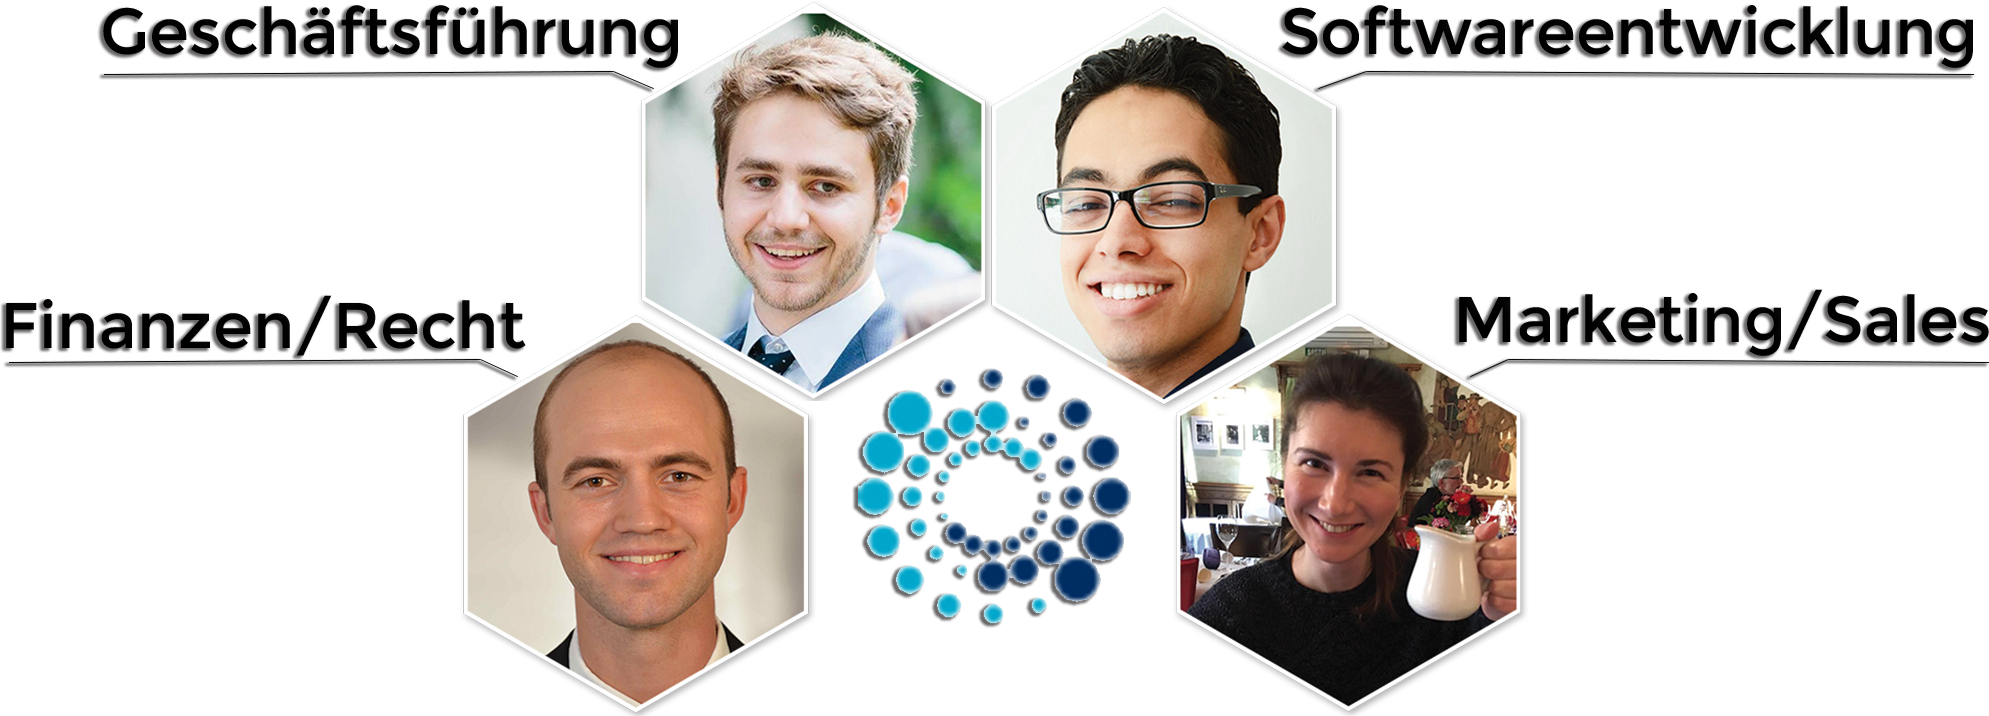
\includegraphics[width=1.0\textwidth]{organigram}}
    \caption{CarBook Organigramm}
    \label{fig:my_label}
\end{figure}

\section{Chancen und Risiken}
Carbook zeichnet sich durch eine einfache Bedienung, hohe Benutzerfreundlichkeit und die Integration unterschiedlicher Anwendungsmöglichkeiten aus (vgl. Kapitel 3). Dennoch gibt es Möglichkeiten zur Verbesserung und Stolpersteine, die bei der Unternehmensgründung und anschließender Einführung in den Markt zu beachten sind.\\ \\
Um diese Möglichkeiten und Gefahren möglichst früh zu erkennen und zu nutzen bzw. zu umgehen, werden im Folgenden mithilfe einer SWOT – Analyse interne Stärken (Strengths) und Schwächen (Weaknesses) den externen Chancen (Opportunities) und Risiken (Threats) gegenübergestellt.\\
\begin{figure}
    \centering
    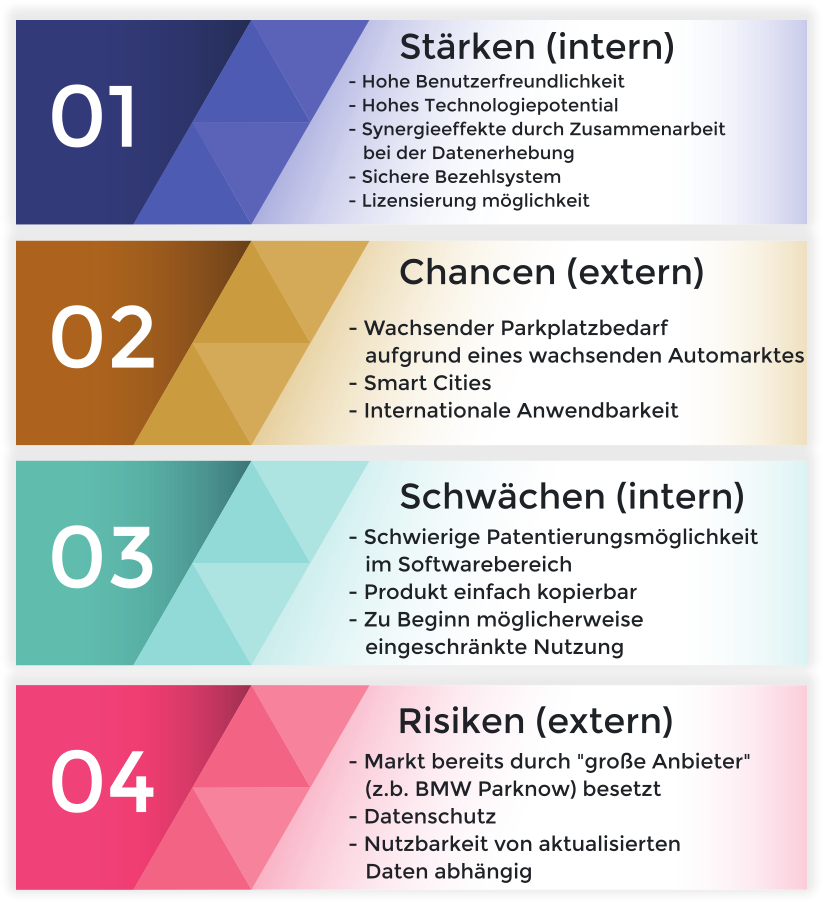
\includegraphics[width=1.0\textwidth]{risiken}
    \caption{Chancen und Risiken}
    \label{fig:risiken}
\end{figure}\\
Bei der \emph{SWOT} – Analyse zeigt sich, dass besonders die einfache Bedienung und die Integration unterschiedlicher Anwendungsmöglichkeiten (Parkplatzfinder, Vermietung, Bezahlung, Informationsbereitstellung) Stärken des Produktes darstellen. Chancen ergeben sich besonders durch den ständig wachsenden Parkplatzbedarf in Städten und die Möglichkeit, Carbook auch auf eine internationale Ebene auszuweiten.\\ \\
Im europäischen Raum und besonders in Deutschland kann es unter Umständen schwierig sein, für eine Softwareanwendung wie Carbook ein geeignetes Patent anzumelden und Patentschutz zu erhalten. Daher besteht die Möglichkeit, dass nach der Markteinführung ähnliche bis identische Apps entwickelt werden, die eine Konkurrenz für Carbook darstellen. Zudem ist zu beachten, dass bereits große Unternehmen wie \emph{BMW} oder der \emph{ADAC} sich mit der Entwicklung von Software beschäftigt haben, die die Parkplatzsuche erleichtern sollen. Des Weiteren hat der Daten- und Verbraucherschutz in Deutschland einen hohen Stellenwert und darf beim Umgang mit sensiblen (also persönlichen) Daten nicht unterschätzt werden.\\ \\
Alles in Allem ist es also wichtig, dass die Chancen und Möglichkeiten von Carbook voll ausgenutzt werden und sichergestellt wird, dass die bereitgestellten Informationen stets aktuell und brauchbar sind. Dies gewährleistet eine ständig wachsende Community und eine hohe Nutzerzufriedenheit.




\vfill
\textit{Made with \ding{170} by CarBook} \autocite{acknow}
\end{document}